%!TEX program = xelatex
\documentclass[12pt, a4paper]{article}

\usepackage[dvipsnames]{xcolor}

\usepackage{fancyhdr}
\usepackage{extramarks}
\usepackage{amsmath}
\usepackage{empheq}
\usepackage{amsthm}
\usepackage{amsfonts}
\usepackage{tikz}
\usepackage{tikz-3dplot}
\usepackage[plain]{algorithm}
\usepackage{algpseudocode}

\usepackage{ctex}
\usepackage{upgreek}
\usepackage{indentfirst}
\usepackage{wrapfig}
\usepackage{subfigure}
\usepackage{pgfplots}
\usepgfplotslibrary{patchplots}
\usepgfplotslibrary{colormaps}
\usepgfplotslibrary{colorbrewer}
\pgfplotsset{compat=1.18}
\usetikzlibrary{automata,positioning,shapes.geometric,arrows.meta,patterns,calc}
\numberwithin{equation}{section}
\CTEXoptions[today=old]

%
% Basic Document Settings
%

\topmargin=-0.25in
\evensidemargin=0in
\oddsidemargin=0in
\textwidth=6.5in
\textheight=9.2in
\headsep=0.25in

\linespread{1.1}

\pagestyle{fancy}
\lhead{\hmwkAuthorName}
\chead{\hmwkClass : \hmwkTitle}
\rhead{\firstxmark}
\lfoot{\lastxmark}
\cfoot{\thepage}

\renewcommand\headrulewidth{0.4pt}
\renewcommand\footrulewidth{0.4pt}

\setlength{\parindent}{2em}  % 2em代表首行缩进两个字符

%
% Create Problem Sections
%

\newcommand{\enterProblemHeader}[1]{
    \nobreak\extramarks{}{Problem \arabic{#1} continued on next page\ldots}\nobreak{}
    \nobreak\extramarks{Problem \arabic{#1} (continued)}{Problem \arabic{#1} continued on next page\ldots}\nobreak{}
}

\newcommand{\exitProblemHeader}[1]{
    \nobreak\extramarks{Problem \arabic{#1} (continued)}{Problem \arabic{#1} continued on next page\ldots}\nobreak{}
    \stepcounter{#1}
    \nobreak\extramarks{Problem \arabic{#1}}{}\nobreak{}
}

% \setcounter{secnumdepth}{0}
\newcounter{partCounter}
\newcounter{homeworkProblemCounter}
\setcounter{homeworkProblemCounter}{0}
% \nobreak\extramarks{Problem \arabic{homeworkProblemCounter}}{}\nobreak{}

%
% Homework Problem Environment
%
% This environment takes an optional argument. When given, it will adjust the
% problem counter. This is useful for when the problems given for your
% assignment aren't sequential. See the last 3 problems of this template for an
% example.
%
\newenvironment{homeworkProblem}[1][-1]{
    \ifnum#1>0
        \setcounter{homeworkProblemCounter}{#1}
    \fi
    \section{Problem \arabic{homeworkProblemCounter}}
    \setcounter{partCounter}{1}
    \enterProblemHeader{homeworkProblemCounter}
}{
    \exitProblemHeader{homeworkProblemCounter}
}

%
% Homework Details
%   - Title
%   - Due date
%   - Class
%   - Section/Time
%   - Instructor
%   - Author
%

\newcommand{\hmwkTitle}{The Method of Differentiation of Multivariate Functions and Its Applications}
\newcommand{\hmwkClass}{Advanced Mathematics}
\newcommand{\hmwkClassTime}{}
\newcommand{\myUniversiy}{Wuhan University}
\newcommand{\hmwkAuthorName}{\textbf{Lai Wei}}

%
% Title Page
%

\title{
    \vspace{2in}
    \textmd{\textbf{\hmwkClass:\ \hmwkTitle}}\\
    \vspace{0.4in}
    \large{\textit{\myUniversiy}}
    \vspace{3in}
}

\author{\hmwkAuthorName}
\date{\today}

\renewcommand{\part}[1]{\textbf{\large Part \Alph{partCounter}}\stepcounter{partCounter}\\}

%
% Various Helper Commands
%

% Useful for algorithms
\newcommand{\alg}[1]{\textsc{\bfseries \footnotesize #1}}

% % For derivatives
% \newcommand{\deriv}[1]{\frac{\mathrm{d}}{\mathrm{d}x} (#1)}

% For partial derivatives
% \newcommand{\pderiv}[2]{\frac{\partial}{\partial #1} (#2)}

% Integral dx
\newcommand{\dx}{\mathrm{d}x}

% Alias for the Solution section header
\newcommand{\solution}{\textbf{\large Solution}}

% Probability commands: Expectation, Variance, Covariance, Bias
\newcommand{\E}{\mathrm{E}}
\newcommand{\Var}{\mathrm{Var}}
\newcommand{\Cov}{\mathrm{Cov}}
\newcommand{\Bias}{\mathrm{Bias}}

% 我的newcommand
\newcommand{\degree}{^{\circ}}
\newcommand{\arrow}{-{Stealth[length=4mm,width=2mm]}}
\newcommand{\rmd}{\mathrm{d}}
\newcommand{\deriv}[2]{\frac{\rmd #1}{\rmd #2}}
\renewcommand{\parallel}{\mathrel{/\mskip-2.5mu/}}
\newcommand{\pderiv}[2]{\frac{\partial #1}{\partial #2}}
\newcommand{\parallelogram}{
	\mathord
    {\text
        {
			\tikz[baseline]
			\draw (0,.1ex) -- (.8em,.1ex) -- (1em,1.6ex) -- (.2em,1.6ex) -- cycle;
        }
    }
}

\begin{document}

\maketitle

\pagebreak

% 设置页码格式是罗马数字
\pagenumbering{roman}

% 生成目录
\tableofcontents

\pagebreak

% 设置页码格式是阿拉伯数字
\pagenumbering{arabic}

\pagebreak

\section{多元函数的基本概念}

\subsection{平面点集}

\subsubsection{坐标平面}

    建立了坐标系的平面。二元有序实数组\(\left(x,y\right)\)
    的全体,即$\mathbf{R}^2=\mathbf{R} \times \mathbf{R}=\{(x, y) 
    \mid x, y \in \mathbf{R}\}$就表示坐标平面。

\subsubsection{平面点集}

    坐标平面上具有某种性质\(P\)的点的几何,称作平面点集,记作

    \[
        E = \left\{\left(x,y\right) \mid \left(x,y\right)
        \text{具有某种性质}P\right\}
    \]

\subsubsection{邻域}

    设\(P_{0}\left(x_0,y_0\right)\)是\(xOy\)平面上一点,
    \(\delta\)是某一正数,与点\(P_{0}\left(x_0,y_0\right)\)
    距离小于\(\delta\)的点\(P\left(x,y\right)\)的全体,称为
    \(P_{0}\)的\(\delta\)邻域,记作\(U\left(P_0,\delta\right)\),
    即

    \[
        U\left(P_0,\delta\right) = \left\{\left(x,y\right)
        \mid \left|PP_0\right| < \delta\right\}
    \]

    或

    \[
        U\left(P_0,\delta\right) = \left\{\left(x,y\right)
        \mid \sqrt{\left(x-x_0\right)^2 + \left(y-y_0\right)^2} < \delta\right\}
    \]

    \textbf{注意}

    \begin{enumerate}
        \item 点\(P_0\)的去心邻域,记作$\stackrel{\circ}{U}\left(P_0, \delta\right)$,即
            $$
                \stackrel{\circ}{U}\left(P_0, \delta\right)=\left\{P\mid0<\left|P P_0\right|<\delta\right\}
            $$
        \item 若不强调\(\delta\),也可记作\(U\left(P_0\right)\),
            \(\stackrel{\circ}{U}\left(P_0\right)\)
    \end{enumerate}

    利用点与点集的关系,可知

    若有一点\(P \in \mathbf{R}^2\),任意点集\(E \subset \mathbf{R}^2\)

    \begin{enumerate}
        \item 内点:\(\exists U\left(P\right)\),使\(U\left(P\right) \subset E\),
            则\(P\)为\(E\)的内点。
        \item 外点:\(\exists U\left(P\right)\),使\(U\left(P\right) \cap E = \phi\),
            则\(P\)为\(E\)的内点。
        \item 边界点:\(\forall U\left(P\right)\),若\(U\left(P\right)\)
            即有属于\(E\)的点,又有不属于\(E\)的点,则\(P\)为\(E\)的边界点。
        \item \(E\)的边界:\(E\)的边界点的全体,记作\(\partial E\)
    \end{enumerate}

\subsubsection{聚点}

    如果对于任意给定的\(\delta>0\),点\(P\)的去心邻域
    \(\stackrel{\circ}{U}\left(P,\delta\right)\)内总有\(E\)
    中的点,那么称\(P\)是\(E\)的聚点。

    例如,若\(E = \left\{\left(x,y\right) \mid
    1 < x^2+y^2 \leq 2\right\}\)。则\(x^2+y^2=1\)
    和\(x^2+y^2=2\)都是\(E\)的聚点。

\subsubsection{由点集所属类的特征分类}

    \begin{enumerate}
        \item 开集:若点集\(E\)中的所有点都是\(E\)的内点,则称\(E\)为开集;
        \item 闭集:若点集\(E\)的边界\(\partial E \in E\),则称\(E\)为闭集。
    \end{enumerate}

    例如,\(\left\{\left(x,y\right) \mid 1 < x^2+y^2 < 2\right\}\)为开集,
    \(\left\{\left(x,y\right) \mid 1 \leq x^2+y^2 \leq 2\right\}\)为闭集,\\
    \(\left\{\left(x,y\right) \mid 1 < x^2+y^2 \leq 2\right\}\)

    \begin{figure}[htbp]
        \centering
        \subfigure[]
        {
            \begin{minipage}[b]{.3\linewidth}
                \centering
                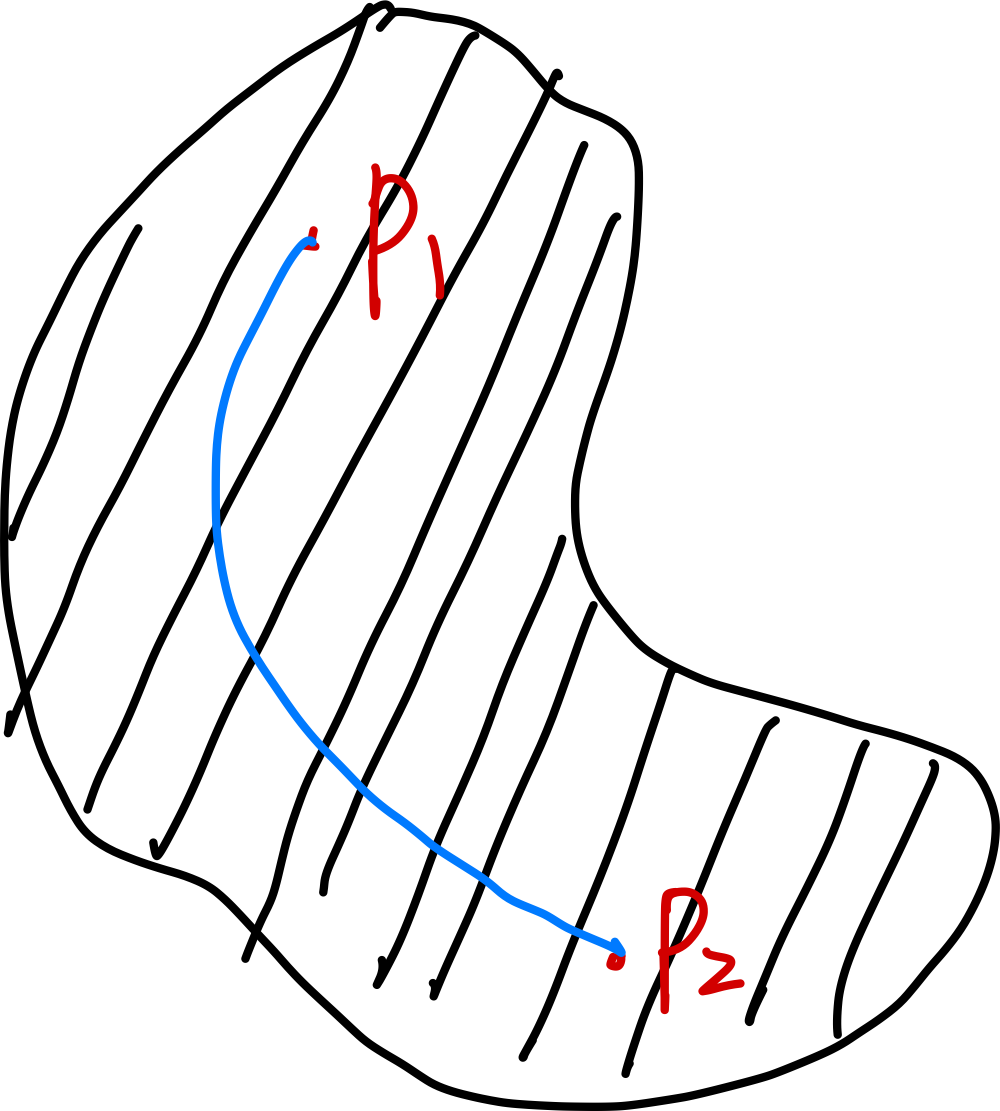
\includegraphics[scale=0.08]{"Chapter 09 images/pic1.png"}
            \end{minipage}
        }
        \subfigure[]
        {
             \begin{minipage}[b]{.3\linewidth}
                \centering
                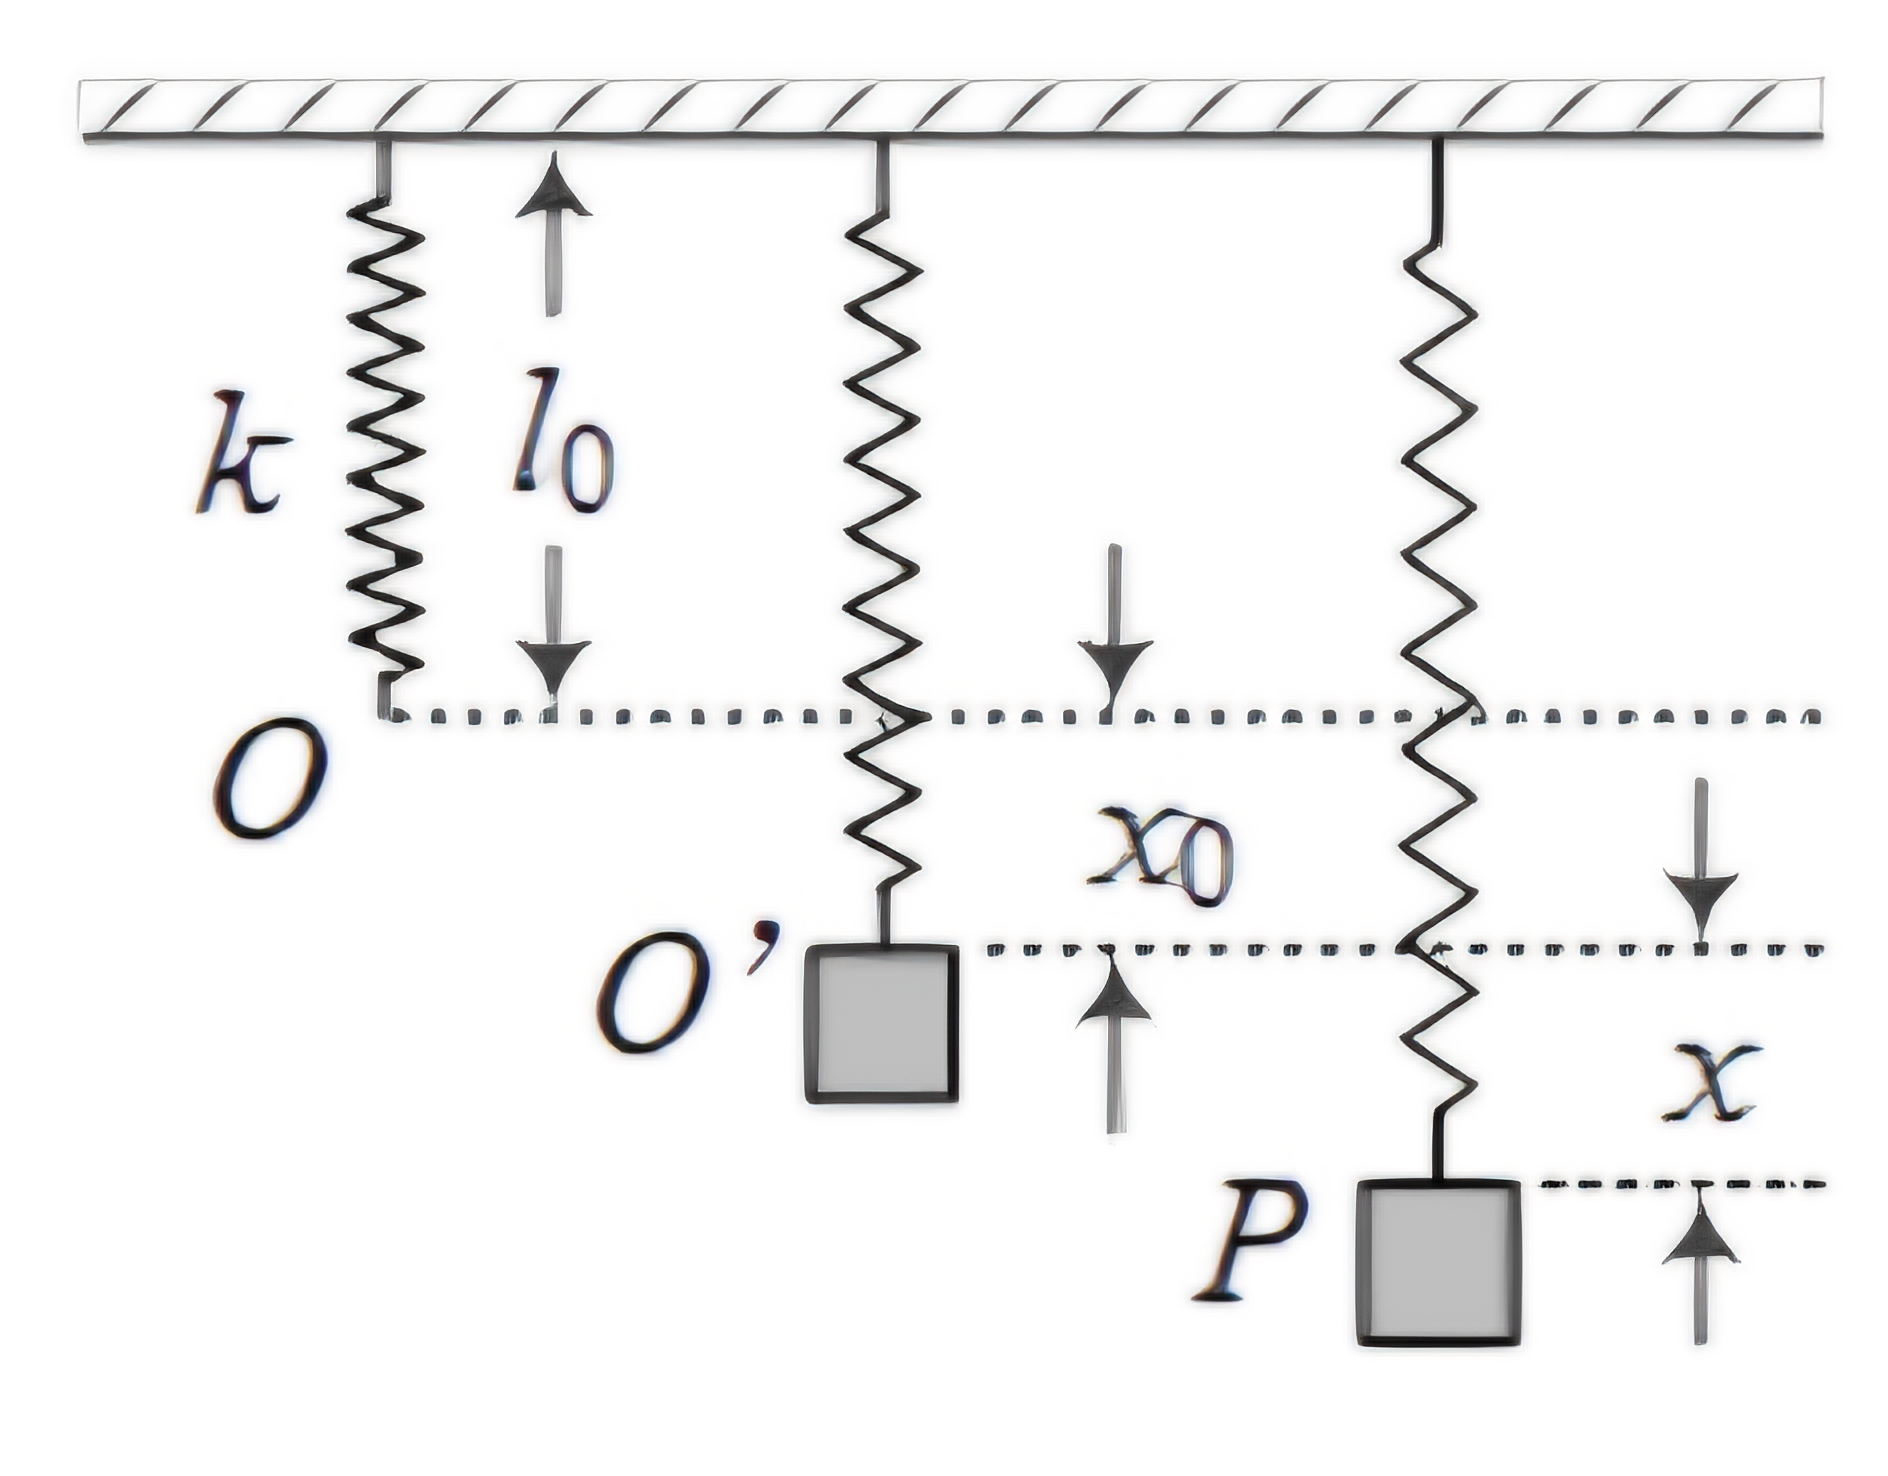
\includegraphics[scale=0.08]{"Chapter 09 images/pic2.jpg"}
            \end{minipage}
        }
    \end{figure}

    \begin{enumerate}
        \item 连通集:如上图(a);
        \item 非连通集:如上图(b)。
    \end{enumerate}

    \begin{enumerate}
        \item 开区域(也简称区域):连通的开集;
        \item 闭区域:开区域连同其边界一起构成的点集。
    \end{enumerate}

    如\(\left\{\left(x,y\right) \mid 1 < x^2+y^2 < 2\right\}\)
    为(开)区域;\(\left\{\left(x,y\right) \mid 1 \leq x^2+y^2 \leq 2\right\}\)
    为闭区域。

    \begin{enumerate}
        \item 有界集:对于集合\(E\),若\(\exists r > 0\),使\(E \subset U\left(0,r\right)\),
            则称\(E\)是有界的。(就是说能找到一个“圆”把集合\(E\)包裹起来)
        \item 无界集:若一个集合不是有界集,则称其为无界集。
    \end{enumerate}

    \begin{figure}[htbp]
        \centering
        \subfigure
        {
        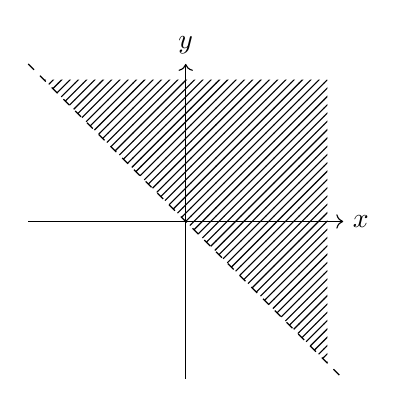
\begin{tikzpicture}
            \coordinate[label=right:$x$] (x) at (2,0);
            \coordinate[label=above:$y$] (y) at (0,2);
            \draw[->] (-2,0) -- (x);
            \draw[->] (0,-2) -- (y);
            \draw[dashed, domain=-2:2] plot(\x,{-\x});
            \fill[pattern=north east lines] (-1.8,1.8) -- (1.8,1.8) -- (1.8,-1.8);
        \end{tikzpicture}
        }
        \subfigure
        {
        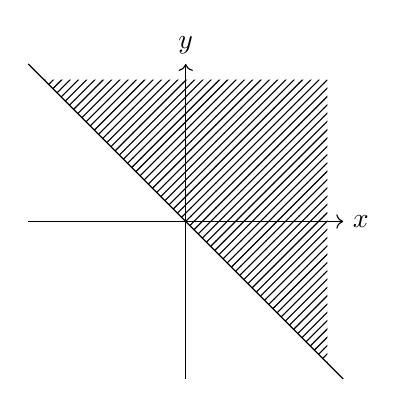
\begin{tikzpicture}
            \coordinate[label=right:$x$] (x) at (2,0);
            \coordinate[label=above:$y$] (y) at (0,2);
            \draw[->] (-2,0) -- (x);
            \draw[->] (0,-2) -- (y);
            \draw[domain=-2:2] plot(\x,{-\x});
            \fill[pattern=north east lines] (-1.8,1.8) -- (1.8,1.8) -- (1.8,-1.8);
        \end{tikzpicture}
        }
    \end{figure}

    例如,\(\left\{\left(x,y\right) \mid x + y > 0\right\}\)为无界开区域;
    \(\left\{\left(x,y\right) \mid x + y \geq 0\right\}\)为无界闭区域。

\subsection{多元函数的概念}

    \subsubsection{二元函数}

    设\(D\)是\(\mathbf{R}^2\)的一个非空子集,称映射\(f: D \rightarrow \mathbf{R}\)为定义在\(D\)上的二元函数,
    通常记为

    \begin{equation}
        z = f\left(x,y\right),\; \left(x,y\right) \in D
    \end{equation}

    或

    \begin{equation}
        z = f\left(P\right),\; P \in D
    \end{equation}

    \subsubsection{值域}

    上述定义中,与自变量\(x\)和y\(\)的一对值(即二元有序实数组)\(\left(x,y\right)\) 相对应的因变量\(z\)的值,
    也称为\(f\)在点\(\left(x,y\right)\)处的函数值,记作\(f\left(x,y\right)\),即\(z=f\left(x,y\right)\)
    函数值\(f\left(x,y\right)\)的全体所构成的集合为函数\(f\)的值域,记作\(f\left(D\right)\),即

    \begin{align}
        f\left(D\right) = \left\{z \mid z=f\left(x,y\right),\; \left(x,y\right) \in D\right\}
    \end{align}

    \subsubsection{推广}

    三元函数:\(u = f\left(x,y,z\right),\; \left(x,y,z\right) \in D\);

    \(n\)元函数:\(u = f\left(x_1,x_2,x_3,\ldots,x_n\right),\; \left(x_1,x_2,x_3,\ldots,x_n\right) \in D\)

    \subsubsection{自然定义域}

    使算式有意义的点的集合。
    
    例如\(z = \ln \left(x+y\right)\)的自然定义域为
    \(D = \left\{\left(x,y\right) \mid x + y > 0\right\}\)。\(z = \arcsin \left(x+y\right)\)
    的自然定义域为\(D = \left\{\left(x,y\right) \mid x^2 + y^2 \leq 1\right\}\)。

    \subsubsection{二元函数的图形}

    设函数\(z=f\left(x,y\right)\)的定义域为\(D\)。对于任意取定的点\(P(x,y) \in D\),
    对应的函数值为\(z=f\left(x,y\right)\)。这样,以\(x\)为横坐标,\(y\)为纵坐标和
    \(z=f\left(x,y\right)\)为竖坐标在空间就确定一点\(M\left(x,y,z\right)\)。
    当\(x,y\)遍取\(D\)上的一切点时,得到一个空间点集

    \begin{align}
        \left\{\left(x,y,z\right) \mid z=f\left(x,y\right),\; \left(x,y\right) \in D\right\}
    \end{align}
    
    这个点集称为二元函数\(z=f\left(x,y\right)\)的图形,通常我们也说二元函数的图形是一张曲面。

    例如,由空间解析几何知道,线性函数$z=ax+by+c$
    的图形是一张平面,而函数$z=x^2+y^2$的图形是旋转抛物面。

\subsection{多元函数的极限}

    如果在\(P\left(x,y\right) \rightarrow P_0\left(x_0,y_0\right)\)(即\(\left|PP_0\right| =
    \sqrt{\left(x-x_0\right)^2 + \left(y-y_0\right)^2} \rightarrow 0\))过程中,对应的函数值
    无限接近于一个确定的常数\(A\),那么就说\(A\)是函数\(f\left(x,y\right)\)当
    \(\left(x,y\right) \rightarrow \left(x_0,y_0\right)\)时的极限。

    \textbf{定义}:“\(\varepsilon - \delta\)”语言

    设二元函数 $f(P)=f(x, y)$ 的定义域为 $D$,$P_0\left(x_0, y_0\right)$
    是$D$的聚点。如果存在常数$A$,对于任意给定的正数$\varepsilon$,总存在正数$\delta$,
    使得当点$P(x, y) \in D \cap \ddot{U}\left(P_0, \delta\right)$ 时,都有

    \begin{equation}
        \left|f(P)-A\right|=\left|f(x, y)-A\right|<\varepsilon
    \end{equation}

    成立,那么就称常数\(A\)为函数\(f\left(x,y\right)\)当\(\left(x,y\right) \rightarrow \left(x_0,y_0\right)\)
    的极限,记作

    \begin{equation}
        \lim _{P \rightarrow P_0} f(P)=A \quad
    \end{equation}

    或

    \begin{equation}
        f(P) \rightarrow A\left(P \rightarrow P_0\right)
    \end{equation}

    \textbf{注意}:

    \begin{enumerate}
        \item \(P_0\)是\(D\)的聚点;
        \item 证明过程中,核心在于寻找\(\delta = \delta\left(\varepsilon\right)\);
        \item 与一元函数不同,\(P \rightarrow P_0\)是指\(P\)以任何方式趋近\(P_0\);
        \item 若\(P\)以不同方式趋近于\(P_0\),\(f\left(p\right)\)趋近于不同值,则可以断定\(f\left(p\right)\)当\(P \rightarrow P_0\)时的极限不存在。
    \end{enumerate}

\subsection{多元函数的连续性}

\subsubsection{连续性的定义}

    设二元函数\(f\left(P\right) = f\left(x,y\right)\)的定义域为\(D\),\(P_0\left(x_0,y_0\right)\)
    为\(D\)的聚点,且\(P_0 \in D\),如果

    \begin{align}
        \lim_{\left(x,y\right) \rightarrow \left(x_0,y_0\right)}f\left(x,y\right) = f\left(x_0,y_0\right)
    \end{align}

    那么称\(f\left(P\right)\)在点\(P_0\left(x_0,y_0\right)\)连续。

    \textbf{注意}:若\(f\left(x,y\right)\)在\(D\)的每一个点都是连续的,则称\(f\left(x,y\right)\)在上\(D\)为连续的。

\subsubsection{间断点的定义}

    设二元函数\(f\left(x,y\right)\)的定义域为\(D\),\(P_0\left(x_0,y_0\right)\)
    为\(D\)的聚点,如果函数\(f\left(x,y\right)\)在\(P_0\left(x_0,y_0\right)\)\\
    点不连续,那么就称\(P_0\left(x_0,y_0\right)\)为函数\(f\left(x,y\right)\)的间断点。

\subsubsection{连续函数的运算}

    一元函数中关于极限的运算法划,对于多元函数仍然适用。根据多元函数的极限运算法则,
    可以证明多元连续函数的和、差、积仍为连续函,连续函数的商在分母不为零出仍连续;
    多元连续函数的复合函数仍然是连续函数。

\subsubsection{多元初等函数}

    与一元初等函数相类似,多元初等函数是指可用一个式子表示的多元函数,这
    个式子是由常数及具有不同自变量的一元基本初等函数经过有限次的四则运算和
    复合运算而得到的。例如\(\frac{x + x^2 + y^2}{1+y^2}\)、
    \(\sin\left(x+y\right)\)、\(e^{x^2 + y^2 + z^2}\)等都是多元初等函数。
    
\subsubsection{有界闭区域上多元函数连续函数的性质}

    \begin{enumerate}
        \item (\textbf{有界性与最大值最小值定理})有界闭区域\(D\)上连续的多元函数,必定在\(D\)上有
            上界,且能取得它的最大值和最小值。\\
            也就是说,若\(P\)在有界闭区域\(D\)上连续,则必定存在常数\(M>0\),使得对一切\(P \in D\)
            有\(\left|f\left(D\right)\right| \leq M\);且存在\(P_1,P_2 \in D\),使得
            $$
                f\left(P_1\right)=\max \{f(P) \mid P \in D\},\; f\left(P_2\right)=\min \{f(P) \mid P \in D\}
            $$
        \item (\textbf{介值定理})在有界闭区域\(D\)上连续的多元函数必取得介于最大值和最小值之间的任何值。
        \item (\textbf{一致连续性定理})在有界闭区域\(D\)上连续的多元函数必定在\(D\)上一致连续。\\
            也就是说,若\(f\left(P\right)\)在有界闭区域\(D\)上连续,则对任意给定的正数\(\varepsilon\),
            总存在正数\(\delta\),使得对于\(D\)上任意两点\(P_1\)、\(P_2\),只要当\(\left|P_1P_2\right| < \varepsilon\)
            时,都有
            $$
                \left|f\left(P_1\right) - f\left(P_2\right)\right| < \varepsilon
            $$
            成立。
    \end{enumerate}

\subsection{例题}

\subsubsection{Problem 1}

    设\(f\left(x,y\right) = \left(x^2+y^2\right)\sin \dfrac{1}{x^2+y^2}\),求证

    \[
        \lim_{\left(x,y\right) \rightarrow \left(x_0,y_0\right)}f\left(x,y\right) = 0
    \]
    \vspace{1em}

    \textbf{Solution}
    \vspace{1em}

    \(f\left(x,y\right)\)的定义域为\(D = \mathbf{R}^2 \backslash \left\{\left(0,0\right)\right\}\),
    点\(O\left(0,0\right)\)为\(D\)的聚点。

    而$\left|f(x, y)-0\right|=\left|f(x, y)\right|=
    \left|\left(x^2+y^2\right) \sin \dfrac{1}{y+x^2}\right| \leq x^2+y^2$

    对\(\forall \varepsilon > 0\)要使$\left|f(x, y)-0\right| \leq x^2+y^2 < \varepsilon$
    成立,取$\delta = \sqrt{\varepsilon}$,则\(0 < \sqrt{x^2+y^2} < \delta\)时,
    有$\left|f(x, y)-0\right| < \varepsilon$。

    于是
    
    \[
        \lim_{\left(x,y\right) \rightarrow \left(x_0,y_0\right)}f\left(x,y\right) = 0
    \]

\subsubsection{Problem 2}

    求证函数

    $$
        f(x, y)= \begin{cases}\dfrac{x y}{x^2+y^2}, & x^2+y^2 \neq 0 \\ 0, & x^2+y^2=0\end{cases}
    $$

    当$\left(x,y\right) \rightarrow \left(0,0\right)$时的极限不存在。
    \vspace{1em}

    \textbf{Solution}
    \vspace{1em}

    显然,当\(P\left(x,y\right)\)沿\(x\)轴趋近于点\(\left(0,0\right)\)时,

    $$
        \lim_{\substack{x, y \rightarrow(0,0) \\ y=0}} f(x, y)=\lim_{x \rightarrow 0} f(x, 0)=\lim _{x \rightarrow 0} 0=0 ;
    $$

    当\(P\left(x,y\right)\)沿直线\(y = kx\)趋近于点\(\left(0,0\right)\)时,

    $$
        \lim_{\substack{(x, y) \rightarrow(0,0) \\ y=k x}} \frac{x y}{x^2+y^2}=\lim_{x \rightarrow 0} \frac{k x^2}{x^2+k^2 x^2}=\frac{k}{1+k^2},
    $$

    显然它是随着\(k\)的值的不同而改变的。

    所以原函数当$\left(x,y\right) \rightarrow \left(0,0\right)$时的极限不存在。

\subsubsection{Problem 3}

    求

    $$
        \lim_{\left(x,y\right) \rightarrow \left(0,2\right)} \frac{\sin\left(xy\right)}{x}
    $$
    \vspace{1em}

    \textbf{Solution}
    \vspace{1em}

    \begin{align*}
        \text{原式} &= \lim_{\left(x,y\right) \rightarrow \left(0,2\right)} \frac{\sin\left(xy\right)}{xy} \cdot y \\
        &=\lim_{xy \rightarrow 0} \frac{\sin\left(xy\right)}{xy} \cdot \lim_{y\rightarrow 2}y \\
        &= 1 \times 2 \\
        &= 2
    \end{align*}

\section{偏导数}

\subsection{偏导数的定义及其计算法}

\subsubsection{定义}

    设函数\(z=f\left(x,y\right)\)在点\(\left(x_0,y_0\right)\)的某一邻域内有定义,
    当\(y\)固定在\(y_0\)而\(x\)在\(x_0\)处有增量\\ \(\Delta x\)时,相应的函数有增量

    $$
        f\left(x_0+\Delta x, y_0\right)-f\left(x_0, y_0\right)
    $$

    如果

    \begin{equation}
        \lim _{\Delta x \rightarrow 0} \frac{f\left(x_0+\Delta x, y_0\right)-f\left(x_0, y_0\right)}{\Delta x}
        \label{9-4-1}
    \end{equation}

    存在,那么称此极限为函数\(z=f\left(x,y\right)\)在点\(\left(x_0,y_0\right)\)处\textbf{对\(x\)的偏导数},记作

    $$
        \left.\frac{\partial z}{\partial x}\right|_{\substack{x=x_0 \\ y=y_0}},\;
        \left.\frac{\partial f}{\partial x}\right|_{\substack{x=x_0 \\ y=y_0}},\;
        \left.z_x\right|_{\substack{x=x_0 \\ y=y_0}}\; \text{或}\;
        f_x\left(x_0, y_0\right) \text {. (1) }
    $$

    例如,方程\ref{9-4-1}可以表为

    \begin{equation}
        f_x\left(x_0, y_0\right)=\lim _{\Delta x \rightarrow 0} \frac{f\left(x_0+\Delta x, y_0\right)-f\left(x_0, y_0\right)}{\Delta x}
    \end{equation}

    类似地,函数\(z=f\left(x,y\right)\)在点\(\left(x_0,y_0\right)\)处\textbf{对\(y\)的偏导数}定义为

    \begin{equation}
        \lim _{\Delta y \rightarrow 0} \frac{f\left(x_0, y_0+\Delta y\right)-f\left(x_0, y_0\right)}{\Delta y}
    \end{equation}

    记作

    $$
        \left.\frac{\partial z}{\partial y}\right|_{\substack{x=x_0 \\ y=y_0}},\;
        \left.\frac{\partial f}{\partial y}\right|_{\substack{x=x_0 \\ y=y_0}},\;
        \left.z_y\right|_{\substack{x=x_0 \\ y=y_0}}\; \text{或}\;
        f_y\left(x_0, y_0\right)
    $$

    如果函数\(z=f\left(x,y\right)\)在区域\(D\)内每一点\(\left(x,y\right)\)处对\(x\)的偏导数都存在,
    那么这个偏导数就是\(x\)、\(y\)的函数,它就称为函数\(z=f\left(x,y\right)\)\textbf{对自变量\(x\)的偏导函数},
    记作

    $$
        \pderiv{z}{x},\;
        \pderiv{f}{x},\;
        z_x\; \text{或}\;
        f_x\left(x, y\right)
    $$

    类似地,可以定义函数\(z=f\left(x,y\right)\)\textbf{对自变量\(y\)的偏导函数},
    记作

    $$
        \pderiv{z}{y},\;
        \pderiv{f}{y},\;
        z_y\; \text{或}\;
        f_y\left(x, y\right)
    $$

    由概念可知,函数\(z=f\left(x,y\right)\)在点\(\left(x_0,y_0\right)\)处对\(x\)的偏导数
    \(f_x\left(x_0, y_0\right)\)显然就是偏导函数\(f_x\left(x, y\right)\)在点\(\left(x_0,y_0\right)\)
    处的函数值;\(f_y\left(x_0, y_0\right)\)就是偏导函数\(f_y\left(x, y\right)\)在点
    \(\left(x_0,y_0\right)\)处的函数值。

\subsubsection{偏导数的求法}

    求\(\pderiv{f}{x}\)时,只要把\(y\)暂时看作常量而对\(x\)求导数;
    求\(\pderiv{f}{y}\)时,只要把\(x\)暂时看作常量而对\(y\)求导数。

    推广:三元函数\(u=f\left(x,y,z\right)\)在点\(\left(x,y,z\right)\)
    处对\(x\)的偏导数定义为

    \begin{equation}
        f_x(x, y, z)=\lim _{\Delta x \rightarrow 0} \frac{f(x+\Delta x, y, z)-f(x, y, z)}{\Delta x}
    \end{equation}

    \textbf{注意}:

    \begin{enumerate}
        \item \(z=f\left(x,y\right)\)的偏导数有2个:\(\pderiv{z}{x}\) 、\(\pderiv{z}{y}\),
            \(u=f\left(x,y,z\right)\)的偏导数有3个:\(\pderiv{u}{x}\) 、\(\pderiv{u}{y}\) 、\(\pderiv{u}{z}\);
        \item \(\pderiv{z}{x}\)是一个整体、一个符号。
    \end{enumerate}


\subsubsection{偏导数的几何意义}

    \begin{wrapfigure}{r}{4cm}
        \centering
        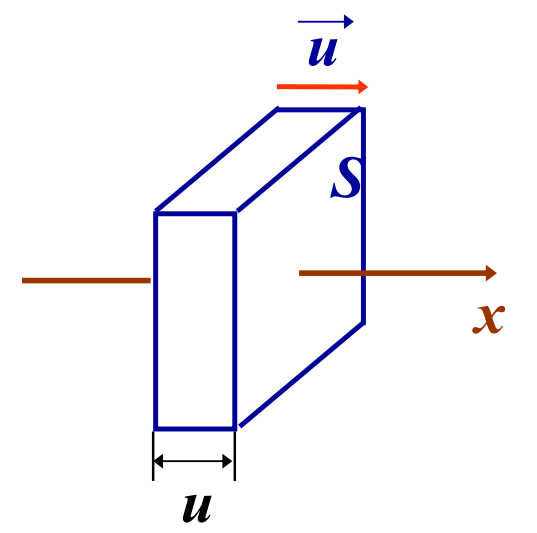
\includegraphics[scale=0.15]{"Chapter 09 images/pic3.jpg"}
        % \caption{}
        \label{pic9-3}
    \end{wrapfigure}

    设\(M_0\left(x_0,y_0,f\left(x_0,y_0\right)\right)\)为曲面\(z=f\left(x,y\right)\)上的一点,
    过\(M_0\)作平面\(y=y_0\),截此曲面得一曲线,此曲线在平面\(y=y_0\)上的方程为
    \(z=f\left(x,y_0\right)\),
    则导数\(\left.\dfrac{\rmd}{\rmd x} f\left(x,y_0\right)\right|_{x=x_0}\),
    即偏导数\(f_x\left(x_0,y_0\right)\),就是这曲线在点\(M_0\)处的切线\(M_0T_x\)
    对\(x\)轴的斜率(如右图所示)。同样,偏导数\(f_y\left(x_0,y_0\right)\)
    的几何意义是曲面被平面\(x=x_0\)所截得的曲线在点\(M_0\)处的切线\(M_0T_y\)
    对\(y\)轴的斜率。
    \vspace{1em}

    \textbf{注意}:

    对多元函数,若函数连续,则偏导数\textbf{不}一定存在;若偏导数存在,
    则函数也\textbf{不}一定连续。例如,函数

    $$
        z=f(x, y)= \begin{cases}\frac{x y}{x^2+y^2}, & x^2+y^2 \neq 0 \\ 0, & x^2+y^2=0\end{cases}
    $$

    在\(\left(0,0\right)\)处是不连续的,而\(f_x\left(0,0\right)=0\),\(f_y\left(0,0\right)=0\),
    即函数在\(\left(0,0\right)\)处的偏导数存在。

\subsection{高阶偏导数}

    设函数\(z=f\left(x,y\right)\)在区域\(D\)内具有偏导数

    $$
        \pderiv{z}{x}=f_x\left(x,y\right),\; \pderiv{z}{y}=f_y\left(x,y\right)
    $$

    于是在\(D\)内\(f_x\left(x,y\right)\),\(f_y\left(x,y\right)\)都是\(x\),\(y\)
    的函数。如果这两个函数的偏导数也存在,那么称它们是函数\(z=f\left(x,y\right)\)
    的\textbf{二阶偏导数}。按照对变量求导次序的不同有下列四个二阶偏导数:

    \begin{align}
        \begin{aligned}
            & \frac{\partial}{\partial x}\left(\frac{\partial z}{\partial x}\right)=\frac{\partial^2 z}{\partial x^2}=f_{x x}(x, y) \\
            & \frac{\partial}{\partial y}\left(\frac{\partial z}{\partial x}\right)=\frac{\partial^2 z}{\partial x \partial y}=f_{x y}(x, y) \\
            & \frac{\partial}{\partial x}\left(\frac{\partial z}{\partial y}\right)=\frac{\partial^2 z}{\partial y \partial x}=f_{y x}(x, y) \\
            & \frac{\partial}{\partial y}\left(\frac{\partial z}{\partial y}\right)=\frac{\partial^2 z}{\partial y^2}=f_{y y}(x, y)
        \end{aligned}
    \end{align}
    
    其中第二、三个偏导数称为\textbf{混合偏导数}。同样可得三阶、四阶……以及\(n\)阶偏导数。二阶以及二阶以上的偏导数统称为
    \textbf{高阶偏导数}。

    \textbf{定理 \quad} 如果函数\(z=f\left(x,y\right)\)的两个二阶混合偏导数相等,即\(\frac{\partial^2 z}{\partial y \partial x}\)
    及\(\frac{\partial^2 z}{\partial x \partial y}\)在区域\(D\)内连续,那么在该区域这两个二阶混合偏导数必相等。

    换句话说,二阶混合偏导数在连续的条件下与求导的次序无关。推广:高阶混合偏导数在偏导数连续的条件下也与求导的次序无关。

\subsection{例题}

\subsubsection{Problem 1}

    证明函数\(u=\dfrac{1}{r}\)满足方程

    $$
        \frac{\partial^2 u}{\partial x^2}+\frac{\partial^2 u}{\partial y^2}+\frac{\partial^2 u}{\partial z^2}=0
    $$

    其中\(r=\sqrt{x^2+y^2+z^2}\)。
    \vspace{1em}

    \textbf{Solution}
    \vspace{1em}

    $$
        \begin{aligned}
        & \frac{\partial u}{\partial x}=-\frac{1}{r^2} \frac{\partial r}{\partial x}=-\frac{1}{r^2} \cdot \frac{x}{r}=-\frac{x}{r^3}, \\
        & \frac{\partial^2 u}{\partial x^2}=-\frac{1}{r^3}+\frac{3 x}{r^4} \cdot \frac{\partial r}{\partial x}=-\frac{1}{r^3}+\frac{3 x^2}{r^5}
        \end{aligned}
    $$

    因为函数关于自变量的对称性,所以

    $$
        \frac{\partial^2 u}{\partial y^2}=-\frac{1}{r^3}+\frac{3 y^2}{r^5}, \quad \frac{\partial^2 u}{\partial z^2}=-\frac{1}{r^3}+\frac{3 z^2}{r^5} .
    $$

    因此,

    $$
        \frac{\partial^2 u}{\partial x^2}+\frac{\partial^2 u}{\partial y^2}+\frac{\partial^2 u}{\partial z^2}=
        -\frac{3}{r^3}+\frac{3\left(x^2+y^2+z^2\right)}{r^5}=-\frac{3}{r^3}+\frac{3 r^2}{r^5}=0
    $$
    \vspace{1em}

    \textbf{注:\quad}例中的方程叫做\textbf{拉普拉斯 (Laplace) 方程},它是数学物理方法中的一种很重要的方程。

\section{全微分}

    \textbf{实质}:寻找多元函数增量的一种\textbf{线性近似}表达。(局部)

\subsection{全微分的定义}

\subsubsection{偏增量、偏微分}

    由偏导数的定义知道,二元函数对某个自变量的偏导数表示当另一个自变量固定时,
    因变量相对于该自变最的变化率。根据一元函数微分学中增量与微分的关系,可得

    $$
        \begin{aligned}
            & f(x+\Delta x, y)-f(x, y) \approx f_x(x, y) \Delta x \\
            & f(x, y+\Delta y)-f(x, y) \approx f_y(x, y) \Delta y
        \end{aligned}
    $$

    上面两式的左端分别叫做二元函数对\(x\)和对\(y\)的偏增量,
    而右端分别叫做二元函数对\(x\)\\和对\(y\)的偏微分。

\subsubsection{全增量}

    设函数\(z=f\left(x,y\right)\)在点\(P\left(x, y\right)\)的某邻域内有定义,
    \(P^{\prime}\left(x+\Delta x,y+\Delta y\right)\)为这邻域内任意一点,则称这两点的函数值之差
    \(f\left(x+\Delta x,y+\Delta y\right)-f\left(x,y\right)\)为函数在点点\(P\)
    对应于自变量增量\(\Delta x\)和\(\Delta y\)的全增量,记作\(\Delta z\),即

    \begin{align}
        \Delta z=f(x+\Delta x, y+\Delta y)-f(x, y)
    \end{align}

\subsubsection{全微分的定义}

    设函数\(z=f\left(x,y\right)\)在点\(\left(x, y\right)\)的某邻域内有定义,
    如果函数在点\(\left(x, y\right)\)的全增量

    $$
        \Delta z=f(x+\Delta x, y+\Delta y)-f(x, y)
    $$

    可表示为

    \begin{align}
        \Delta z=A \Delta x+B \Delta y+o(\rho)
    \end{align}

    其中\(A\)和\(B\)不依赖于\(\Delta x\)和\(\Delta y\)而仅与\(x\)和\(y\)有关,
    \(\rho = \sqrt{\left(\Delta x\right)^2+\left(\Delta y\right)^2}\),
    那么称函数\(z=f\left(x,y\right)\)在点\(\left(x, y\right)\)\textbf{可微分},
    而\(A\Delta x + B\Delta y\)称为函数\(z=f\left(x,y\right)\)在点\(\left(x, y\right)\)
    的\textbf{全微分},记作\(\rmd z\),即

    $$
        \mathrm{d} z=A \Delta x+B \Delta y
    $$

    如果函数在区域\(D\)内各点处都可微分,那么称函数在\(D\)内可微分。

    如果函数\(z=f\left(x,y\right)\)在点\(\left(x, y\right)\)可微分,
    那么这函数在该点必定连续。
    
\subsubsection{例题}

    若已知如果函数\(f\left(x,y\right)\)在点\(\left(0, 0\right)\)处连续,且

    $$
        \lim _{(x, y) \rightarrow(0,0)} \frac{f(x, y)-3 x+4 y}{\sqrt{x^2+y^2}}=0
    $$

    问:\(f\left(x,y\right)\)在点\(\left(0, 0\right)\)处是否可微?若可微,求

    $$
        \rmd f\left|_{\left(0,0\right)}\right.
    $$
    \vspace{1em}

    \textbf{Solution}
    \vspace{1em}

    由题意

    $$
        \lim _{(x, y) \rightarrow(0,0)}\left[f(x, y)-3 x+4 y\right]=0
    $$

    所以

    $$
        \lim _{(x, y) \rightarrow(0,0)} f(x, y)=0
    $$

    又函数\(f\left(x,y\right)\)在点\(\left(0, 0\right)\)处连续,由上式得

    $$
        f\left(0,0\right)=0
    $$

    由原式

    $$
        f(x, y)-3 x+4 y=o(\rho)
    $$

    即

    $$
        f\left(x,y\right) - f\left(0,0\right) = 3 x-4 y+o(\rho),\quad
        \rho = \sqrt{x^2+y^2}
    $$

    亦即

    $$
        f\left(\Delta x,\Delta y\right) - f\left(0,0\right) = 3 \Delta x-4 \Delta y+o(\rho),\quad
        \rho = \sqrt{\left(\Delta x\right)^2+\left(\Delta y\right)^2}
    $$

    由定义,函数\(f\left(x,y\right)\)在点\(\left(0, 0\right)\)处可微,且

    $$
        \rmd f\left|_{\left(0,0\right)}\right. = 3 \Delta x-4 \Delta y
    $$

\subsection{可微分的条件}

    \textbf{定理1(必要条件)}:如果函数\(z=f\left(x,y\right)\)在点\(\left(x, y\right)\)可微分,
    那么函数在点\(\left(x, y\right)\)的偏导数\(\pderiv{z}{x}\)和\(\pderiv{z}{y}\)必定存在,
    且函数\(z=f\left(x,y\right)\)在点\(\left(x, y\right)\)的全微分为

    \begin{equation}
        \mathrm{d} z=\frac{\partial z}{\partial x} \Delta x+\frac{\partial z}{\partial y} \Delta y
    \end{equation}

    利用定义判断可微的方法:

    \begin{enumerate}
        \item 先求\(f^{\prime}_x\left(x_0,y_0\right)\)、\(f^{\prime}_y\left(x_0,y_0\right)\),若不存在,则不可微;
        \item 判断
            $$
                \lim _{\substack{\Delta x \rightarrow 0 \\ \Delta y \rightarrow 0}}
                \frac{\Delta z-f_x^{\prime}\left(x_0, y_0\right) \Delta x-f_y^{\prime}\left(x_0, y_0\right) \Delta y}
                {\sqrt{(\Delta x)^2+(\Delta y)^2}}=0
            $$
            是否成立。其中,

            $$
                \Delta z =f\left(x_0+\Delta x, y_0+\Delta y\right)-f\left(x_0, y_0\right)
            $$
            
            若成立,则可微;反之,则不可微。
    \end{enumerate}

    \textbf{注意}:与一元函数不同,各偏导数的存在只是全微分存在的必要条件而不是充分条件。

    \textbf{定理2(充分条件)}:如果函数\(z=f\left(x,y\right)\)的偏导数\(\pderiv{z}{x}\)、\(\pderiv{z}{y}\)
    在点\(\left(x, y\right)\)连续,那么函数在该点可微分。

    偏导连续,即

    $$
        \lim _{\substack{x \rightarrow x_0 \\ y \rightarrow y_0}} f_x^{\prime}(x, y)=f_x^{\prime}\left(x_0, y_0\right)
    $$

    (\(f_x^{\prime}\)在点\(\left(x_0, y_0\right)\)处连续)

    $$
        \lim _{\substack{x \rightarrow x_0 \\ y \rightarrow y_0}} f_y^{\prime}(x, y)=f_y^{\prime}\left(x_0, y_0\right)
    $$

    (\(f_y^{\prime}\)在点\(\left(x_0, y_0\right)\)处连续)

\subsection{全微分公式}

    \begin{equation}
        \rmd z=\frac{\partial z}{\partial x} \rmd x+\frac{\partial z}{\partial y} \rmd y
    \end{equation}

    特别地,

    \begin{equation}
        \left.d z\right|_{\left(x_0, y_0\right)}=
        f_x^{\prime}\left(x_0, y_0\right) \cdot d x+f_y^{\prime}\left(x_0, y_0\right) \cdot d y
    \end{equation}

    \textbf{推广}:

    \begin{equation}
        \rmd u=\frac{\partial u}{\partial x} \rmd x+\frac{\partial u}{\partial y} \rmd y+\frac{\partial u}{\partial z} \rmd z
    \end{equation}

\section{多元复合函数求导法则}

\subsection{中间变量为一元函数情形}

    \textbf{定理1}:如果函数\(u=\varphi\left(t\right)\)及\(v=\psi\left(t\right)\)都在点\(t\)可导,
    函数\(z=f\left(u,v\right)\)在对应点\(\left(u,v\right)\)\\具有连续偏导数,那么复合函数\(z=
    f\left[\varphi\left(t\right), \psi\left(t\right)\right]\)在点\(t\)可导,且有

    \begin{equation}
        \frac{\mathrm{d} z}{\mathrm{~d} t}=\frac{\partial z}{\partial u} \frac{\mathrm{~d} u}{\mathrm{~d} t}
        +\frac{\partial z}{\partial v} \frac{\mathrm{~d} v}{\mathrm{~d} t}
    \end{equation}
    \vspace{1em}

    复合关系图:

    \[
        \tikzset{every picture/.style={line width=0.75pt}} %set default line width to 0.75pt        
        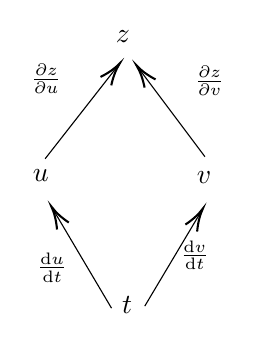
\begin{tikzpicture}[x=0.75pt,y=0.75pt,yscale=-1,xscale=1]
        %uncomment if require: \path (0,300); %set diagram left start at 0, and has height of 300
        %Straight Lines [id:da10650359767783146] 
        \draw    (278.14,129.29) -- (312.91,84.86) ;
        \draw [shift={(314.14,83.29)}, rotate = 128.05] [color={rgb, 255:red, 0; green, 0; blue, 0}][line width=0.75]
            (10.93,-3.29) .. controls (6.95,-1.4) and (3.31,-0.3) .. (0,0) .. controls (3.31,0.3) and (6.95,1.4) .. (10.93,3.29);
        %Straight Lines [id:da08370320770247508] 
        \draw    (355.14,128.29) -- (323.34,85.89) ;
        \draw [shift={(322.14,84.29)}, rotate = 53.13] [color={rgb, 255:red, 0; green, 0; blue, 0}][line width=0.75]
            (10.93,-3.29) .. controls (6.95,-1.4) and (3.31,-0.3) .. (0,0) .. controls (3.31,0.3) and (6.95,1.4) .. (10.93,3.29);
        %Straight Lines [id:da6078309854266968] 
        \draw    (326.14,200.29) -- (353.12,155) ;
        \draw [shift={(354.14,153.29)}, rotate = 120.78] [color={rgb, 255:red, 0; green, 0; blue, 0}][line width=0.75]
            (10.93,-3.29) .. controls (6.95,-1.4) and (3.31,-0.3) .. (0,0) .. controls (3.31,0.3) and (6.95,1.4) .. (10.93,3.29);
        %Straight Lines [id:da19651881359339796] 
        \draw    (310.14,201.29) -- (282.16,154.01) ;
        \draw [shift={(281.14,152.29)}, rotate = 59.38] [color={rgb, 255:red, 0; green, 0; blue, 0}][line width=0.75]    
            (10.93,-3.29) .. controls (6.95,-1.4) and (3.31,-0.3) .. (0,0) .. controls (3.31,0.3) and (6.95,1.4) .. (10.93,3.29);
        % Text Node
        \draw (311,66.4) node [anchor=north west][inner sep=0.75pt] {$z$};
        \draw (271,133.4) node [anchor=north west][inner sep=0.75pt] {$u$};
        \draw (350,134.4) node [anchor=north west][inner sep=0.75pt] {$v$};
        \draw (314,194.4) node [anchor=north west][inner sep=0.75pt] {$t$};
        \draw (270,82.4) node [anchor=north west][inner sep=0.75pt] [font=\footnotesize] {$\frac{\partial z}{\partial u}$};
        \draw (349,83.4) node [anchor=north west][inner sep=0.75pt] [font=\footnotesize] {$\frac{\partial z}{\partial v}$};
        \draw (273,173.4) node [anchor=north west][inner sep=0.75pt] [font=\footnotesize] {$\frac{\mathrm{d} u}{\mathrm{d} t}$};
        \draw (342,167.4) node [anchor=north west][inner sep=0.75pt] [font=\footnotesize] {$\frac{\mathrm{d} v}{\mathrm{d} t}$};
        \end{tikzpicture}
    \]

    \textbf{证}

    由于\(z=f\left(x,y\right)\)在\(\left(u,v\right)\)可微,故

    $$
        \Delta z=\frac{\partial f}{\partial u} \cdot \Delta u+\frac{\partial f}{\partial v} \cdot \Delta v+o(\rho), \rho=\sqrt{(\Delta u)^2+(\Delta v)^2}
    $$

    上式两端同时除以\(\Delta t\):

    $$
        \begin{aligned}
            \frac{\Delta z}{\Delta t} & =\frac{\partial f}{\partial u} \cdot \frac{\Delta u}{\Delta t}+\frac{\partial t}{\partial v} \cdot \frac{\Delta v}{\Delta t}+\frac{o(\rho)}{\Delta t} \\
            & =\frac{\partial f}{\partial t} \cdot \frac{\Delta u}{\Delta t}+\frac{\partial f}{\partial v} \cdot \frac{\Delta v}{\Delta t}+\frac{o(\rho)}{\rho} \cdot \frac{\sqrt{(\Delta u)^2+(\Delta v)^2}}{\Delta t} \\
            & =\frac{\partial f}{\partial u} \cdot \frac{\Delta u}{\Delta t}+\frac{\partial f}{\partial v} \cdot \frac{\partial v}{\Delta t}+\frac{o(\rho)}{\rho} \cdot \sqrt{\left(\frac{\Delta u}{\Delta t}\right)^2+\left(\frac{\Delta v}{\Delta t}\right)^2}
        \end{aligned}
    $$

    由于\(u\),\(v\)是可导的,故二者连续,从而:

    当\(\Delta t \rightarrow 0\)时,\(\Delta u \rightarrow 0\),\(\Delta v \rightarrow 0\);

    从而也有\(\rho \rightarrow 0\),于是\(\dfrac{o(\rho)}{\rho} \rightarrow 0\)。

    令\(\Delta t \rightarrow 0\),得全导数

    $$
        \deriv{z}{t}=\frac{\partial z}{\partial u} \frac{\mathrm{~d} u}{\mathrm{~d} t}+\frac{\partial z}{\partial v} \frac{\mathrm{~d} v}{\mathrm{~d} t} .
    $$
    
    证毕。

    推广:若$z=f\left[\varphi(t), \psi(t), \omega(t)\right]$,则全导数

    \begin{equation}
        \deriv{z}{t}=\frac{\partial f}{\partial u} \cdot \deriv{u}{t}+\frac{\partial f}{\partial v} \cdot \deriv{v}{t}+\frac{\partial f}{\partial w} \cdot \deriv{w}{t}
    \end{equation}

\subsection{中间变量为多元函数情形}

    \textbf{定理2}:如果函数\(u=\varphi\left(x,y\right)\)及\(v=\psi\left(x,y\right)\)都在点\(\left(x,y\right)\)
    具有对\(x\)及对\(y\)的偏导数,函数\(z=f\left(u,v\right)\)在对应点\(\left(u,v\right)\)具有连续偏导数,
    那么复合函数\(z=f\left[\varphi\left(x,y\right), \psi\left(x,y\right)\right]\)在点\\\(\left(x,y\right)\)
    的两个偏导数都存在,且有

    \begin{equation}
        \frac{\partial z}{\partial x}=\frac{\partial z}{\partial u} \frac{\partial u}{\partial x}
        +\frac{\partial z}{\partial v} \frac{\partial v}{\partial x}
    \end{equation}

    \begin{equation}
        \frac{\partial z}{\partial y}=\frac{\partial z}{\partial u} \frac{\partial u}{\partial y}
        +\frac{\partial z}{\partial v} \frac{\partial v}{\partial y}
    \end{equation}

    类似地,设\(u=\varphi\left(x,y\right)\)、\(v=\psi\left(x,y\right)\)、\(w=\omega\left(x,y\right)\)都在点
    \(\left(x,y\right)\)具有对\(x\)及对\(y\)的偏导数,函数$f\left(u,v,w\right)$在对应点\(\left(u,v,w\right)\)具有
    连续偏导数,则复合函数
    
    $$
        z=f\left[\varphi(x,y), \psi(x,y), \omega(x,y)\right]
    $$

    在点\(\left(x,y\right)\)的两个偏导数都存在,且可用下列公式计算:

    \begin{equation}
        \frac{\partial z}{\partial x}=\frac{\partial z}{\partial u} \frac{\partial u}{\partial x}+
        \frac{\partial z}{\partial v} \frac{\partial v}{\partial x}+\frac{\partial z}{\partial w} \frac{\partial w}{\partial x}
    \end{equation}

    \begin{equation}
        \frac{\partial z}{\partial y}=\frac{\partial z}{\partial u} \frac{\partial u}{\partial y}+
        \frac{\partial z}{\partial v} \frac{\partial v}{\partial y}+\frac{\partial z}{\partial w} \frac{\partial w}{\partial y}
    \end{equation}

\subsection{混合情形}

    \textbf{定理3}:如果函数\(u=\varphi\left(x,y\right)\)在点\(\left(x,y\right)\)具有\(x\)对\(y\)的偏导数,函数
    \(v=\psi\left(y\right)\)在\(y\)点可到,函数\(z=f\left(u,v\right)\)在对应点\(\left(u,v\right)\)具有连续偏导数,
    那么复合函数\(z=f\left[\varphi\left(x,y\right), \psi\left(t\right)\right]\)在点\(\left(x,y\right)\)都存在,
    且有

    \begin{equation}
        \frac{\partial z}{\partial x}=\frac{\partial z}{\partial u} \frac{\partial u}{\partial x}
    \end{equation}

    \begin{equation}
        \frac{\partial z}{\partial y}=\frac{\partial z}{\partial u} \frac{\partial u}{\partial y}+\frac{\partial z}{\partial v} \frac{\mathrm{~d} v}{\mathrm{~d} y}
    \end{equation}

    其他情形,如函数\(z=f\left(u, v, x\right)\),\(u=\varphi\left(x,y\right)\),\(v=\psi\left(y\right)\),即
    \(z=f\left[\varphi\left(x,y\right), \psi\left(y\right), x\right]\),则

    \begin{equation}
        \begin{aligned}
            \frac{\partial z}{\partial x} & =\frac{\partial f}{\partial u} \cdot \frac{\partial u}{\partial x}+
            \frac{\partial f}{\partial v} \cdot 0+\frac{\partial f}{\partial x} \cdot 1 \\
            & =\frac{\partial f}{\partial u} \cdot \frac{\partial u}{\partial x}+\frac{\partial f}{\partial x}
        \end{aligned}
    \end{equation}

    \begin{equation}
        \frac{\partial z}{\partial y}=\frac{\partial f}{\partial u} \cdot \frac{\partial u}{\partial y}+\frac{\partial f}{\partial v} \cdot \deriv{v}{y}
    \end{equation}

\subsection{抽象复合函数求偏导}

    为了写法和计算上的方便,引入记号(若有函数\(z=f\left(u,v\right)\)):

    $$
        \begin{aligned}
            \left\{\begin{array}{ll}
                f_u^{\prime} \rightarrow f_1^{\prime}, &f_v^{\prime} \rightarrow f_2^{\prime} \\
                f_{u u}^{\prime \prime} \rightarrow f_{11}^{\prime \prime}, &f_{u v}^{\prime \prime} \rightarrow f_{12}^{\prime \prime} \\
                \ldots
            \end{array}\right.
        \end{aligned}
    $$

\subsection{全微分的形式不变性}

    设函数\(z=f\left(u, v\right)\)具有连续偏导数,且\(u=\varphi\left(x,y\right)\),\(v=\psi\left(x,y\right)\),
    则有全微分

    \begin{equation}
        \begin{aligned}
            \mathrm{d} z&=\frac{\partial z}{\partial u} \mathrm{~d} u+\frac{\partial z}{\partial v} \mathrm{~d} v \\
            &=\left(\frac{\partial z}{\partial u} \frac{\partial u}{\partial x}+\frac{\partial z}{\partial v} \frac{\partial v}{\partial x}\right) \mathrm{d} x+\left(\frac{\partial z}{\partial u} \frac{\partial u}{\partial y}+
                \frac{\partial z}{\partial v} \frac{\partial v}{\partial y}\right) \mathrm{d} y \\
            &=\frac{\partial z}{\partial u}\left(\frac{\partial u}{\partial x} \mathrm{~d} x+\frac{\partial u}{\partial y} \mathrm{~d} y\right)+\frac{\partial z}{\partial v}\left(\frac{\partial v}{\partial x} \mathrm{~d} x
                +\frac{\partial v}{\partial y} \mathrm{~d} y\right) \\
            &=\frac{\partial z}{\partial u} \rmd u+\frac{\partial z}{\partial v} \rmd v
        \end{aligned}
    \end{equation}

    可见,无论\(u\)和\(v\)是自变量还是中间变量,函数\(z=f\left(u,v\right)\)的全微分形式是一样的。
    这个性质叫做\textbf{全微分的形式不变性}。

\section{隐函数的求导公式}

\subsection{隐函数的类型}

\subsubsection{一个方程的情形}

    二元方程:

    \[
        F\left(x,y\right)=0 \Longrightarrow y=y\left(x\right) \text{或} x=x\left(y\right)
    \]
    
    三元方程:

    \[
        F\left(x,y,z\right)=0 \Longrightarrow z=z\left(x,y\right) \text{或} y=y\left(x,z\right)
        \text{或} x=x\left(y,z\right)
    \]
    
\subsubsection{方程组的情形}

    三元方程组:

    $$
        \left\{\begin{array} {l} 
        {F(x,y,z) = 0} \\
        {G(x,y,z) = 0}
        \end{array} \Longrightarrow \left\{\begin{array}{l} 
        {y=y(x)} \\
        {z=z(x)}
        \end{array} \text{或} \left\{\begin{array}{l}
        x=x(y) \\
        z=z(y)
        \end{array}\text{或} \left\{\begin{array}{l}
        x=x(z) \\
        y=y(z)
        \end{array}\right.\right.\right.\right.
    $$

    四元方程组:

    $$
        \left\{\begin{array} {l} 
        {F( x,y,u,v)=0} \\
        {G(x,y,u,v)=0}
        \end{array} \Longrightarrow \left\{\begin{array}{l}
        u=U(x, y) \\
        v=V(x, y)
        \end{array} \quad \cdots
        \right.\right.
    $$

    统一:

    $$
        \text{总变量个数} - \text{方程个数(约束)} = \text{自变量个数}
    $$

\subsection{一个方程的情形}

\subsubsection{定理}

    \textbf{隐函数存在定理1}:设函数\(F\left(x,y\right)\)在点\(P_0\left(x_0,y_0\right)\)的某一邻域内
    具有连续偏导数,且\\\(F\left(x_0,y_0\right)=0\),\(F_y\left(x_0,y_0\right)\neq0\),则方程
    \(F\left(x,y\right)=0\)在点\(\left(x_0,y_0\right)\)的某一邻域内恒能唯一确定一个连续且具有连续导数的函数
    \(y=f\left(x\right)\),它满足条件\(y_0=f\left(x_0\right)\),并有

    \begin{equation}
        \frac{\mathrm{d} y}{\mathrm{~d} x}=-\frac{F_x}{F_y}
        \label{9-5-1}
    \end{equation}

    (交叉对应添负号)

    该定理要求的三个条件:

    \begin{enumerate}
        \item 在点\(P_0\left(x_0,y_0\right)\)的某一邻域内具有连续偏导数;
        \item \(F\left(x_0,y_0\right)=0\);
        \item \(F_y\left(x_0,y_0\right)\neq0\)(\(F_y \neq 0 \Rightarrow y = y(x)\),相应地,
            \(F_x \neq 0 \Rightarrow x = x(y)\))。
    \end{enumerate}

    就方程\ref{9-5-1}作如下推导:

    \[
        \tikzset{every picture/.style={line width=0.75pt}} %set default line width to 0.75pt        
        \begin{tikzpicture}[x=0.75pt,y=0.75pt,yscale=-1,xscale=1]
        %uncomment if require: \path (0,300); %set diagram left start at 0, and has height of 300
        %Straight Lines [id:da8751139333655369] 
        \draw    (163.52,114.26) -- (163.37,149.82);
        \draw [shift={(163.36,151.82)}, rotate = 270] [color={rgb, 255:red, 0; green, 0; blue, 0}][line width=0.75]
            (10.93,-3.29) .. controls (6.95,-1.4) and (3.31,-0.3) .. (0,0) .. controls (3.31,0.3) and (6.95,1.4) .. (10.93,3.29)   ;
        %Straight Lines [id:da425976278970581] 
        \draw    (163.57,179.82) -- (162.13,232.32);
        \draw [shift={(162.07,234.32)}, rotate = 270] [color={rgb, 255:red, 0; green, 0; blue, 0}][line width=0.75]
            (10.93,-3.29) .. controls (6.95,-1.4) and (3.31,-0.3) .. (0,0) .. controls (3.31,0.3) and (6.95,1.4) .. (10.93,3.29)   ;
        % Text Node
        \draw (144.33,91.73) node [anchor=north west][inner sep=0.75pt]    {$F(x,y) =0\ \Longrightarrow y=y(x)$};
        \draw (177,119) node [anchor=north west][inner sep=0.75pt]   [align=left] {关于$\displaystyle x$求导};
        \draw (143.83,145.4) node [anchor=north west][inner sep=0.75pt]    {$F_{x} \cdot 1+F_{y} \ \cdot \dfrac{\mathrm{d} y}{\mathrm{d} x} =0$};
        \draw (177.5,194.5) node [anchor=north west][inner sep=0.75pt]   [align=left] {从中解出$\displaystyle \frac{\mathrm{d} y}{\mathrm{d} x}$};
        \draw (145.83,239.23) node [anchor=north west][inner sep=0.75pt]    {$\dfrac{\mathrm{d} y}{\mathrm{d} x} =-\dfrac{F_{x}}{F_{y}} \ (F_{y} =0)$};
        \end{tikzpicture}
    \]

    隐函数的高阶导数:

    \(\dfrac{\rmd y}{\rmd x}\)再对\(x\)求导数时,\(y\)不能当作常数,应作为\(x\)的函数\(y=y(x)\)对待。

    \vspace{1em}
    \textbf{隐函数存在定理2}(三元方程):设函数\(F\left(x,y,z\right)\)在点\(P_0\left(x_0,y_0,z_0\right)\)的某一邻域内
    具有连续偏导数,且\(F\left(x_0,y_0,z_0\right)=0\),\(F_z\left(x_0,y_0,z_0\right)\neq0\),则方程
    \(F\left(x,y,z\right)=0\)在点\(\left(x_0,y_0,z_0\right)\)\\的某一邻域内恒能唯一确定一个连续且具有连续偏导数的函数
    \(z=f\left(x,y\right)\),它满足条件\(z_0=f\left(x_0,y_0\right)\),并有

    \begin{equation}
        \frac{\partial z}{\partial x}=-\frac{F_x}{F_z}, \frac{\partial z}{\partial y}=-\frac{F_y}{F_z}
        \label{9-5-2}
    \end{equation}

    (交叉对应添负号)

    该定理要求的三个条件:

    \begin{enumerate}
        \item 在点\(P_0\left(x_0,y_0,z_0\right)\)的某一邻域内具有连续偏导数;
        \item \(F\left(x_0,y_0,z_0\right)=0\);
        \item \(F_y\left(x_0,y_0,z_0\right)\neq0\)(\(F_z \neq 0 \Rightarrow z = z(x,y)\),相应地,
            \(F_x \neq 0 \Rightarrow x = x(y,z)\)、\(F_y \neq 0 \Rightarrow y = y(z,x)\))。
    \end{enumerate}

    就方程\ref{9-5-2}作如下推导:
    
    \[
        \tikzset{every picture/.style={line width=0.75pt}} %set default line width to 0.75pt        
        \begin{tikzpicture}[x=0.75pt,y=0.75pt,yscale=-1,xscale=1]
        %uncomment if require: \path (0,300); %set diagram left start at 0, and has height of 300
        %Straight Lines [id:da8751139333655369] 
        \draw    (163.52,114.26) -- (163.37,149.82) ;
        \draw [shift={(163.36,151.82)}, rotate = 270.25] [color={rgb, 255:red, 0; green, 0; blue, 0 }  ][line width=0.75]
            (10.93,-3.29) .. controls (6.95,-1.4) and (3.31,-0.3) .. (0,0) .. controls (3.31,0.3) and (6.95,1.4) .. (10.93,3.29)   ;
        %Straight Lines [id:da425976278970581] 
        \draw    (163.57,179.82) -- (163.78,232.54) ;
        \draw [shift={(163.79,234.54)}, rotate = 269.78] [color={rgb, 255:red, 0; green, 0; blue, 0 }  ][line width=0.75]
            (10.93,-3.29) .. controls (6.95,-1.4) and (3.31,-0.3) .. (0,0) .. controls (3.31,0.3) and (6.95,1.4) .. (10.93,3.29)   ;
        % Text Node
        \draw (144.33,91.73) node [anchor=north west][inner sep=0.75pt]    {$F( x,y,z) =0\ \Longrightarrow z=z( x,y)$};
        \draw (177,119) node [anchor=north west][inner sep=0.75pt]   [align=left] {关于$\displaystyle x$求导};
        \draw (143.33,145.4) node [anchor=north west][inner sep=0.75pt]    {$F_{x} \cdot 1+F_{y} \cdot 0+F_{z} \ \cdot \dfrac{\partial z}{\partial x} =0$};
        \draw (177.5,193) node [anchor=north west][inner sep=0.75pt]   [align=left] {从中解出$\displaystyle \frac{\partial z}{\partial x}$};
        \draw (145.83,239.23) node [anchor=north west][inner sep=0.75pt]    {$\dfrac{\partial z}{\partial x} =-\dfrac{F_{x}}{F_{z}} \ ( F_{z} =0)$};
        \end{tikzpicture}
    \]

    求\(F\left(x,y,z\right)=0\)所确定的函数\(z\)的偏导数的方法:

    \begin{enumerate}
        \item 方程直接关于\(x\)或\(y\)求偏导(\(z\)看作\(x\),\(y\)的函数),解出\(\pderiv{z}{x}\)、\(\pderiv{z}{y}\)(复合函数求导法);
        \item 公式法:求出\(F_x\),\(F_x\),\(F_x\)代入公式。
    \end{enumerate}

\subsubsection{例题}

    \textbf{例1}
    \vspace{1em}

    验证方程\(x^2+y^2-1=0\)在点\(\left(0,1\right)\)的某一邻域内恒能唯一确定一个有连续的导数,
    当\(x=0\),\(y=1\)时的隐函数\(y=f\left(x\right)\),并求这函数的一阶与二阶导数在\(x=0\)
    的值。
    \vspace{1em}

    \textbf{Solution}
    \vspace{1em}

    记\(F\left(x,y\right)=x^2+y^2-1\),

    \begin{enumerate}
        \item 显然\(F\left(x,y\right)\)处处连续且具有偏导数;
        \item \(F\left(0,1\right)=0\);
        \item \(F_y=2y\),所以\(F_y\left(0,1\right)=2\neq0\)。
    \end{enumerate}

    利用隐函数存在定理1,满足条件的隐函数\(y=f\left(x\right)\)存在。

    由

    $$
        F_x=2x,\; F_y = 2y
    $$

    所以

    $$
        \begin{aligned}
            &\frac{\mathrm{d} y}{\mathrm{~d} x}=-\frac{F_x}{F_y}=-\frac{x}{y},\left.\quad
                \frac{\mathrm{~d} y}{\mathrm{~d} x}\right|_{\substack{x=0 \\ y=1}}=0; \\
            & \frac{\mathrm{d}^2 y}{\mathrm{~d} x^2}=-\frac{y-x y^{\prime}}{y^2}=-\frac{y-x\left(-\frac{x}{y}\right)}{y^2}
                =-\frac{y^2+x^2}{y^3}=-\frac{1}{y^3}, \\
            & \left.\frac{\mathrm{~d}^2 y}{\mathrm{~d} x^2}\right|_{x=0}=-1 .
        \end{aligned}
    $$

    \textbf{例2}
    \vspace{1em}

    设\(z=z\left(x,y\right)\)由\(F\left(x-z,y+z\right)=0\)确定,\(F\)可微,求证

    \[
        \pderiv{z}{x} - \pderiv{z}{y} = 1
    \]
    \vspace{1em}

    \textbf{Solution}
    \vspace{1em}

    记\(G\left(x,y,z\right)=F\left(x-z,y+z\right)\),则

    $$
        \begin{aligned}
            & G_x=F_1^{\prime} \cdot(1-0)+F_2^{\prime} \cdot 0=F_1^{\prime} ; \\
            & G_y=F_1^{\prime} \cdot 0+F_2^{\prime} \cdot(1+0)=F_2^{\prime} ; \\
            & G_z=F_1^{\prime} \cdot(0-1)+F_2^{\prime} \cdot(0+1)=F_2^{\prime}-F_1^{\prime} ;
        \end{aligned}
    $$

    所以

    $$
        \begin{aligned}
            & \frac{\partial z}{\partial x}=-\frac{G_x}{G_z}=-\frac{F^{\prime}}{F_2^{\prime}-F_1^{\prime}}=\frac{F_1^{\prime}}{F_1^{\prime}-F_2^{\prime}} \\
            & \frac{\partial z}{\partial y}=-\frac{G_y}{G_z}=-\frac{F_2^{\prime}}{F_2-F_1^{\prime}}=\frac{F_2^{\prime}}{F_1^{\prime}-F_2}
        \end{aligned}
    $$

    代入原式:

    $$
        \text{左边} = \frac{\partial z}{\partial x}-\frac{\partial z}{\partial y}=\frac{F_1^{\prime}-F_2^{\prime}}{F_1^{\prime}-F_2^{\prime}}=1 = \text{右边}
    $$

    证毕。

\subsection{方程组的情形}

\subsubsection{定理}

    \textbf{隐函数存在定理3}:设函数\(F\left(x,y,u,v\right)\)、\(G\left(x,y,u,v\right)\)在点\(P_0\left(x_0,y_0,u_0,v_0\right)\)
    的某一邻域内具有对各个变量的连续偏导数,又\(F\left(x_0,y_0,u_0,v_0\right)=0\),\(G\left(x,y,u,v\right)=0\),
    且偏导数所组成的函数行列式(或称雅可比(Jacobi)式)

    $$
        J=\frac{\partial(F, G)}{\partial(u, v)}=\left|\begin{array}{ll}
        \dfrac{\partial F}{\partial u} & \dfrac{\partial F}{\partial v} \\ \\
        \dfrac{\partial G}{\partial u} & \dfrac{\partial G}{\partial v}
        \end{array}\right|
    $$

    在点\(P_0\left(x_0,y_0,u_0,v_0\right)\)处不为零,则方程组\(F\left(x,y,u,v\right)\)、\(G\left(x,y,u,v\right)\)
    在点\(\left(x_0,y_0,u_0,v_0\right)\)\\的某一邻域内恒能唯一确定一组连续且具有连续偏导数的函数
    \(u=u\left(x,y\right)\),\(v=v\left(x,y\right)\),它们满足条件\(u_0=u\left(x_0,y_0\right)\),
    \(v_0=v\left(x_0,y_0\right)\),并有

    \begin{equation}
        \begin{aligned}
            & \frac{\partial u}{\partial x}=-\frac{1}{J} \frac{\partial(F, G)}{\partial(x, v)}=-\frac{\left|\begin{array}{ll}
            F_x & F_v \\
            G_x & G_v
            \end{array}\right|}{\left|\begin{array}{ll}
            F_u & F_v \\
            G_u & G_v
            \end{array}\right|}, \\
            & \frac{\partial v}{\partial x}=-\frac{1}{J} \frac{\partial(F, G)}{\partial(u, x)}=-\frac{\left|\begin{array}{ll}
            F_u & F_x \\
            G_u & G_x
            \end{array}\right|}{\left|\begin{array}{ll}
            F_u & F_v \\
            G_u & G_v
            \end{array}\right|}, \\
            & \frac{\partial u}{\partial y}=-\frac{1}{J} \frac{\partial(F, G)}{\partial(y, v)}=-\frac{\left|\begin{array}{ll}
            F_y & F_v \\
            G_y & G_v
            \end{array}\right|}{\left|\begin{array}{ll}
            F_u & F_v \\
            G_u & G_v
            \end{array}\right|}, \\
            & \frac{\partial v}{\partial y}=-\frac{1}{J} \frac{\partial(F, G)}{\partial(u, y)}=-\frac{\left|\begin{array}{ll}
            F_u & F_v \\
            G_u & G_y
            \end{array}\right|}{\left|\begin{array}{ll}
            F_u & F_v \\
            G_u & G_v
            \end{array}\right|}.
        \end{aligned}
    \end{equation}

    该定理要求的三个条件:

    \begin{enumerate}
        \item 在点\(P_0\left(x_0,y_0,u_0,v_0\right)\)的某一邻域内具有连续偏导数;
        \item \(F\left(x_0,y_0,u_0,v_0\right)=0\),\(G\left(x,y,u,v\right)=0\);
        \item 函数行列式(或称雅可比(Jacobi)式)
            $$
                J=\frac{\partial(F, G)}{\partial(u, v)}=\left|\begin{array}{ll}
                \dfrac{\partial F}{\partial u} & \dfrac{\partial F}{\partial v} \\ \\
                \dfrac{\partial G}{\partial u} & \dfrac{\partial G}{\partial v}
                \end{array}\right|
            $$
            在点\(P_0\left(x_0,y_0,u_0,v_0\right)\)处不为零
    \end{enumerate}

\subsubsection{例题}

    \textbf{例1}
    \vspace{1em}

    求由$\left\{\begin{array}{l}x+y+z=0 \\ x^2+y^2+z^2=1\end{array}\right.$
    所确定的函数的导数\(\deriv{x}{z}\)、\(\deriv{y}{z}\)。
    \vspace{1em}

    \textbf{Solution}
    \vspace{1em}

    方程组对\(z\)求导

    $$
        \left\{\begin{array}{c}
            \deriv{x}{z}+\deriv{y}{z}+1=0 \\
            2 x \deriv{x}{z}+2 y \deriv{y}{z}+2 z=0
        \end{array}\right.
    $$

    即

    $$
        \left\{\begin{array}{c}
            \deriv{x}{z}+\deriv{y}{z}=-1 \\
            2 x \deriv{x}{z}+2 y \deriv{y}{z}=-2 z
        \end{array}\right.
    $$

    当雅可比行列式

    $$
        J=\left|\begin{array}{cc}
            1 & 1 \\
            2 x & 2 y
        \end{array}\right|=2(y-x) \neq 0
    $$

    时,有

    $$
        \deriv{x}{z}=\frac{\left|\begin{array}{cc}
        -1 & 1 \\
        -2 z & 2 y
        \end{array}\right|}{\left|\begin{array}{cc}
        1 & 1 \\
        2 x & 2 y
        \end{array}\right|}=\frac{2(z-y)}{2(y-x)}=\frac{z-y}{y-x}
    $$

    $$
        \deriv{y}{z}=\frac{\left|\begin{array}{cc}
        1 & -1 \\
        2 x & -2 z
        \end{array}\right|}{\left|\begin{array}{cc}
        1 & 1 \\
        2 x & 2 y
        \end{array}\right|}=\frac{2(x-z)}{2(y-x)}=\frac{x-z}{y-x}
    $$

    \textbf{例1}
    \vspace{1em}

    求由$\left\{\begin{array}{l}x=\mathrm{e}^u+u \sin v \\ y=\mathrm{e}^u-u \cos v\end{array}\right.$
    所确定的函数的导数$\frac{\partial u}{\partial x}, \frac{\partial u}{\partial y},
    \frac{\partial v}{\partial x}, \frac{\partial v}{\partial y}$。
    \vspace{1em}

    \textbf{Solution}
    \vspace{1em}

    原方程组两边求微分,得

    $$
        \left\{\begin{array}{l}
            \mathrm{d} x=\left(\mathrm{e}^u+\sin v\right) \mathrm{d} u+u \cos v \mathrm{~d} v \\
            \mathrm{~d} y=\left(\mathrm{e}^u-\cos v\right) \mathrm{d} u+u \sin v \mathrm{~d} v
        \end{array}\right.
    $$

    当雅可比行列式

    $$
        \left|\begin{array}{ll}
            \mathrm{e}^u+\sin v & u \cos v \\
            \mathrm{e}^u-\cos v & u \sin v
        \end{array}\right|=u \mathrm{e}^u(\sin v-\cos v)+u \neq 0
    $$

    时,有

    $$
        \rmd v =\frac{u \sin v \mathrm{~d} x-u \cos v \mathrm{~d} y}{u \mathrm{e}^u(\sin v-\cos v)+u}=
        \frac{\sin v}{e^u(\sin v-\cos v)+1} \mathrm{~d} x+\frac{-\cos v}{\mathrm{e}^u(\sin v-\cos v)+1} \mathrm{~d} y
    $$

    $$
        \begin{aligned}
            \mathrm{~d} v & =\frac{\left(\mathrm{e}^u+\sin v\right) \mathrm{d} y-\left(\mathrm{e}^u-\cos v\right)
                \mathrm{d} x}{u \mathrm{e}^u(\sin v-\cos v)+u} \\
            &=\frac{\mathrm{e}^u+\sin v}{u \mathrm{e}^u(\sin v-\cos v)+u} \mathrm{~d} y+
                \frac{\cos v-\mathrm{e}^u}{u \mathrm{e}^u(\sin v-\cos v)+u} \mathrm{~d} x
        \end{aligned}
    $$

    所以

    $$
        \frac{\partial u}{\partial x}=\frac{\sin v}{\mathrm{e}^u(\sin v-\cos v)+1}
    $$

    $$
        \frac{\partial u}{\partial y}=\frac{-\cos v}{\mathrm{e}^u(\sin v-\cos v)+1}
    $$

    $$
        \frac{\partial v}{\partial x}=\frac{\cos v-\mathrm{e}^u}{u \mathrm{e}^u(\sin v-\cos v)+u}
    $$

    $$
        \frac{\partial v}{\partial y}=\frac{\mathrm{e}^u+\sin v}{u \mathrm{e}^u(\sin v-\cos v)+u}
    $$

    \textbf{例3}
    \vspace{1em}

    求由$\left\{\begin{array}{l}2 x u+y^2 v=0, \\ y u+3 x v=1,\end{array}\right.$
    所确定的函数的导数$\frac{\partial u}{\partial x}, \frac{\partial u}{\partial y},
    \frac{\partial v}{\partial x}, \frac{\partial v}{\partial y}$。
    \vspace{1em}

    \textbf{Solution}
    \vspace{1em}

    方程组$\left\{\begin{array}{l}2 x u+y^2 v=0, \\ y u+3 x v=1,\end{array}\right.$
    两边关于\(x\)求偏导并整理得

    $$
        \left\{\begin{array}{l}
            2 x \dfrac{\partial u}{\partial x}+y^2 \dfrac{\partial v}{\partial x}=-2 u \\ \\
            y \dfrac{\partial u}{\partial x}+3 x \dfrac{\partial v}{\partial x}=-3 v
        \end{array}\right.
    $$

    当$\left|\begin{array}{cc}2 x & y^2 \\ y & 3 x\end{array}\right|=6 x^2-y^3 \neq 0$时,
    由隐函数求导公式即得

    $$
        \frac{\partial u}{\partial x}=\frac{3 y^2 v-6 x u}{6 x^2-y^3}
    $$

    $$
        \frac{\partial v}{\partial x}=\frac{2 y u-6 x v}{6 x^2-y^3}
    $$

    类似可求得

    $$
        \frac{\partial u}{\partial y}=\frac{y^2 u-6 x y u}{6 x^2-y^3}
    $$

    $$
        \frac{\partial v}{\partial y}=\frac{2 y^2 v-2 x u}{6 x^2-y^3} .
    $$

    \textbf{例4}
    \vspace{1em}

    设\(\varphi\left(u,v\right)\)为可微函数,证明:由方程\(\varphi\left(cx-az, cy-bz\right)=0\)
    所确定的隐函数满足方程\(a \dfrac{\partial z}{\partial x}+b \dfrac{\partial z}{\partial y}\)。
    \vspace{1em}

    \textbf{Solution}
    \vspace{1em}

    令$F(x, y, z)=\varphi(c x-a z, c y-b z)=0$,则

    $$
        F_x^{\prime}=c \varphi_1^{\prime}, \quad F_y^{\prime}=c \varphi_2^{\prime}, \quad F_z^{\prime}=-a \varphi_1^{\prime}-b \varphi_2^{\prime}
    $$

    于是有

    $$
        \frac{\partial z}{\partial x}=\frac{c \varphi_1^{\prime}}{a \varphi_1^{\prime}+b \varphi_2^{\prime}},
        \frac{\partial z}{\partial y}=\frac{c \varphi_2^{\prime}}{a \varphi_1^{\prime}+b \varphi_2^{\prime}}
    $$

    故

    $$
        a \frac{\partial z}{\partial x}+b \frac{\partial z}{\partial y}=
        \frac{a c \varphi_1^{\prime}}{a \varphi_1^{\prime}+b \varphi_2^{\prime}}+
        \frac{b c \varphi_2^{\prime}}{a \varphi_1^{\prime}+b \varphi_2^{\prime}}=c
    $$

\section{多元函数微分学应用}

\subsection{向量值函数及其导数}

    由空间解析几何知道,空间曲线\(\varGamma\)的参数方程为

    \begin{equation}
        \left\{\begin{array}{l}
            x=\varphi(t), \\
            y=\psi(t), \\
            z=\omega(t),
        \end{array} \quad t \in[\alpha, \beta]. \right.
        \label{9-6-1}
    \end{equation}

    方程\ref{9-6-1}也可以写成向量形式。若记

    \begin{align*}
        \overrightarrow{r} = x\overrightarrow{i} + y\overrightarrow{j} + z\overrightarrow{k}, \quad
        \overrightarrow{f}\left(t\right) = \varphi\left(t\right)\overrightarrow{i} +
            \psi\left(t\right)\overrightarrow{j} + \omega\left(t\right)
    \end{align*}

    则方程\ref{9-6-1}就成为向量方程

    \begin{equation}
        \overrightarrow{r} = \overrightarrow{f}\left(t\right),\quad t \in[\alpha, \beta]
    \end{equation}

    \textbf{定义1}:设数集\(D \subset \mathbf{R}\),则称映射\(\overrightarrow{f}: D \rightarrow \mathbf{R}^n\)
    为一元向量值函数,通常记为

    \begin{equation}
        \overrightarrow{r} = \overrightarrow{f}\left(t\right),\quad t \in D
    \end{equation}

    其中数集\(D\)称为函数的定义域,\(t\)称为自变量,\(\overrightarrow{r}\)称为因变量。

    \begin{enumerate}
        \item 一元向量值函数(向量值函数)与普通实值函数(数量函数)的关系:一元向量值函数是对普通一元函数的推广。
            现在,自变量\(t\)依然取实数值,但因变量\(\overrightarrow{r}\)不取实数值,而取值为\(n\)维向量。
        \item 向量值函数的图形:
            $$
                \begin{aligned}
                    \overrightarrow{r}=\overrightarrow{f}(t) & =f_1(t) \overrightarrow{i}+f_2(t) \overrightarrow{j}+f_3(t) \overrightarrow{k} \\
                    & =\left(f_1(t), f_2(t), f_3(t)\right)
                \end{aligned}
            $$
            \[
                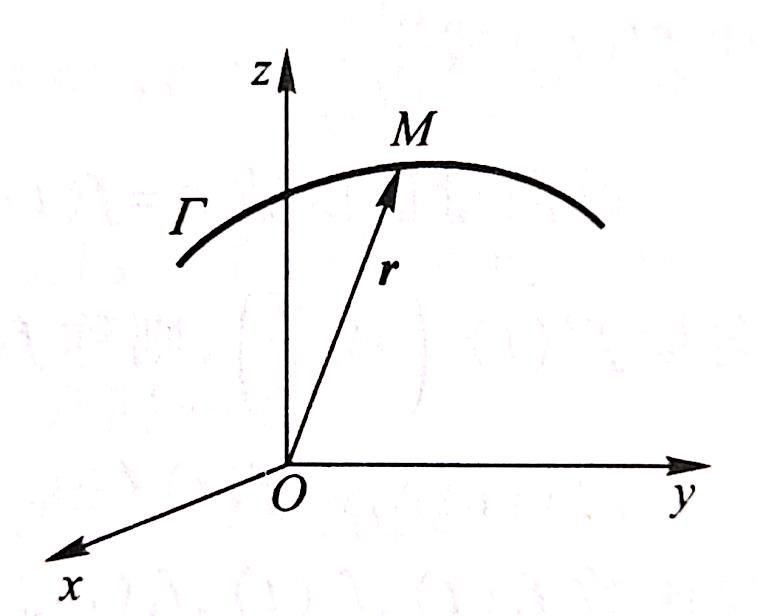
\includegraphics[scale=0.2]{Chapter 09 images/pic4.jpg}
            \]
            若\(\overrightarrow{r} = \overrightarrow{OM}\),则\(M\)的轨迹(记作\(\varGamma\))称为向量值函数
            \(\overrightarrow{r} = \overrightarrow{f}\left(t\right)\)的终端曲线,曲线\(\varGamma\)也称为向量值函数
            \(\overrightarrow{r} = \overrightarrow{f}\left(t\right)\)的图形。
    \end{enumerate}

    \textbf{定义2}:设向量值函数\(\overrightarrow{f}\left(t\right)\)在点\(t\)
    的某一去心邻域内有定义,如果存在一个常向量\(\overrightarrow{r}_0\),对于任意给定的正数\(\varepsilon\)总存在正数
    \(\delta\)使得当\(t\)满足\(0<\left|t-t_0\right|<\delta\)时,对应的函数值\(\overrightarrow{f}\left(t\right)\)
    都满足不等式
    
    \[
        \left|\overrightarrow{f}\left(t\right)-\overrightarrow{r}_0\right| < \varepsilon
    \]

    那么,常向量\(\overrightarrow{r}_0\)就叫做向量值函数\(\overrightarrow{f}\left(t\right)\)
    当\(t \rightarrow t_0\)时的极限,记作
    
    \begin{equation}
        \lim_{t \rightarrow t_0} \overrightarrow{f}(t) = \overrightarrow{r}_0 \quad 
        \text{或} \quad \overrightarrow{f}(t) \rightarrow \overrightarrow{r}_0, t \rightarrow t_0
    \end{equation}

    \begin{enumerate}
        \item 向量值函数\(\overrightarrow{f}\left(t\right)\)当\(t \rightarrow t_0\)
            时的极限存在的充分必要条件是\(f\left(t_1\right)\),\(f\left(t_2\right)\),
            \(f\left(t_3\right)\)当\(t \rightarrow t_0\)时的极限都存在。
        \item 设向量值函数\(\overrightarrow{f}\left(t\right)\)在点\(t_0\)
            的某一去心邻域内有定义,若
            \begin{align}
                \lim_{t \rightarrow t_0}\overrightarrow{f}\left(t\right) = \overrightarrow{f}\left(t_0\right)
            \end{align}
            则称\(\overrightarrow{f}\left(t\right)\)在点\(t_0\)处连续。
    \end{enumerate}

    \textbf{定义2}:设向量值函数\(\overrightarrow{r} = \overrightarrow{f}\left(t\right)\)在点\(t_0\)
    的某一去心邻域内有定义,如果
    
    \begin{equation}
        \lim _{\Delta t \rightarrow 0} \frac{\Delta \overrightarrow{r}}{\Delta t}=
        \lim _{\Delta t \rightarrow 0} \frac{\overrightarrow{f}\left(t_0+\Delta t\right)-\overrightarrow{f}\left(t_0\right)}{\Delta t}
    \end{equation}

    存在,那么就称这个极限向量为向量值函数\(\overrightarrow{r} = \overrightarrow{f}\left(t\right)\)
    在\(t_0\)处的导数或导向量,记作\(\overrightarrow{f}^{\prime}\left(t_0\right)\)或
    \(\left.\dfrac{\rmd \overrightarrow{r}}{\rmd t}\right|_{t=t_0}\)。

    向量函数导数的运算法则如下(\(\overrightarrow{u}\left(t\right)\)、\(\overrightarrow{v}\left(t\right)\)
    是可导的向量值函数,\(\overrightarrow{C}\)是常向量,\(c\)是任一常数,\(\varphi\left(t\right)\)
    是可到的数量函数):

    \begin{enumerate}
        \item $$
                \frac{\mathrm{d}}{\mathrm{~d} t} \overrightarrow{C}=\overrightarrow{0}
            $$
        \item $$
                \frac{\mathrm{d}}{\mathrm{~d} t}[c \overrightarrow{u}(t)]=c \overrightarrow{u}^{\prime}(t)
            $$
        \item $$
                \frac{\mathrm{d}}{\mathrm{~d} t}[\overrightarrow{u}(t) \pm \overrightarrow{v}(t)]=\overrightarrow{u}^{\prime}(t) \pm \overrightarrow{v}^{\prime}(t)
            $$
        \item $$
                \frac{\mathrm{d}}{\mathrm{~d} t}[\varphi(t) \overrightarrow{u}(t)]=
                \varphi^{\prime}(t) \overrightarrow{u}(t)+\varphi(t) \overrightarrow{u}^{\prime}(t)
            $$
        \item $$
                \frac{\mathrm{d}}{\mathrm{~d} t}[\overrightarrow{u}(t) \cdot \overrightarrow{v}(t)]=
                \overrightarrow{u}^{\prime}(t) \cdot \overrightarrow{v}(t)+\overrightarrow{u}(t) \cdot \overrightarrow{v}^{\prime}(t)
            $$
        \item $$
                \frac{\mathrm{d}}{\mathrm{~d} t}[\overrightarrow{u}(t) \times \overrightarrow{v}(t)]=
                \overrightarrow{u}^{\prime}(t) \times \overrightarrow{v}(t)+\overrightarrow{u}(t) \times \overrightarrow{v}^{\prime}(t)
            $$
        \item $$
                \frac{\mathrm{d}}{\mathrm{~d} t} \overrightarrow{u}[\varphi(t)]=\varphi^{\prime}(t) \overrightarrow{u}^{\prime}[\varphi(t)]
            $$
    \end{enumerate}

\subsection{空间曲线的切线与法向量}

\subsubsection{公式}

    设空间曲线\(\varGamma\)的参数方程为

    \begin{equation}
        \left\{\begin{array}{l}
            x=\varphi(t), \\
            y=\psi(t), \\
            z=\omega(t),
        \end{array} \quad t \in[\alpha, \beta]. \right.
        \label{9-6-7}
    \end{equation}

    这里假定\ref{9-6-7}式的三个函数都在\([\alpha, \beta]\)
    上可导,且三个导数不同时为零。

    现要求曲线\(\varGamma\)在其上一点\(M\left(x_0,y_0,z_0\right)\)处的切线及法平面方程。

    设点\(M\)对应的参数为\(t_0\)。记$f(t)=(\varphi(t), \psi(t), \omega(t)), t \in[\alpha, \beta]$。
    则切向量

    $$
        \overrightarrow{T}=\overrightarrow{f}^{\prime}\left(t_0\right)=
        \left(\varphi^{\prime}\left(t_0\right), \psi^{\prime}\left(t_0\right), \omega^{\prime}\left(t_0\right)\right)
    $$

    从而曲线\(\varGamma\)在点\(M\left(x_0,y_0,z_0\right)\)处的切线方程为

    \begin{equation}
        \frac{x-x_0}{\varphi^{\prime}\left(t_0\right)}=
        \frac{y-y_0}{\psi^{\prime}\left(t_0\right)}=\frac{z-z_0}{\omega^{\prime}\left(t_0\right)}
        \label{9-6-8}
    \end{equation}

    于是法平面方程为

    \begin{equation}
        \varphi^{\prime}\left(t_0\right)\left(x-x_0\right)+\psi^{\prime}\left(t_0\right)\left(y-y_0\right)+\omega^{\prime}\left(t_0\right)\left(z-z_0\right)=0
        \label{9-6-9}
    \end{equation}

\subsubsection{其他情形}

    如果空间曲线\(\varGamma\)的方程以

    $$
        \left\{\begin{array}{l}
            y=\varphi(x) \\
            z=\psi(x)
        \end{array}\right.
    $$

    的形式给出,取\(x\)为参数,它就可以表示为参数方程的形式

    $$
        \left\{\begin{array}{l}
            x=x \\
            y=\varphi(x) \\
            z=\psi(x)
        \end{array}\right.
    $$

    如果空间曲线\(\varGamma\)的方程以

    \begin{equation}
        \left\{\begin{array}{l}
            F(x, y, z)=0 \\
            G(x, y, z)=0
        \end{array}\right.
        \label{9-6-10}
    \end{equation}

    的形式给出,\(M\left(x_0,y_0,z_0\right)\)是曲线\(\varGamma\)上一点。
    又设\(F\)、\(G\)为有对各个变量的连续偏导数,且

    $$
        \left.\frac{\partial(F, G)}{\partial(y, z)}\right|_{\left(x_0, y_0, z_0\right)} \neq 0
    $$

    方程\ref{9-6-10}满足隐函数存在定理条件,确定一组函数\(\varphi(x)\)、\(\psi(x)\),则

    $$
        \left\{\begin{array}{l}
            F[x, \varphi(x), \psi(x)] \equiv 0 \\
            G[x, \varphi(x), \psi(x)] \equiv 0
        \end{array}\right.
    $$

    两端分别对\(x\)求全导数,得

    $$
        \left\{\begin{array}{l}
            \dfrac{\partial F}{\partial x}+\dfrac{\partial F}{\partial y} \dfrac{\mathrm{~d} y}{\mathrm{~d} x}+
                \dfrac{\partial F}{\partial z} \dfrac{\mathrm{~d} z}{\mathrm{~d} x}=0 \\ \\
            \dfrac{\partial G}{\partial x}+\dfrac{\partial G}{\partial y} \dfrac{\mathrm{~d} y}{\mathrm{~d} x}+
                \dfrac{\partial G}{\partial z} \dfrac{\mathrm{~d} z}{\mathrm{~d} x}=0
        \end{array}\right.
    $$

    故可解得

    $$
        \frac{\mathrm{d} y}{\mathrm{~d} x}=\varphi^{\prime}(x)=\frac{\left|\begin{array}{ll}
        F_z & F_x \\
        G_z & G_x
        \end{array}\right|}{\left|\begin{array}{ll}
        F_y & F_z \\
        G_y & G_z
        \end{array}\right|}
    $$

    $$
        \frac{\mathrm{d} z}{\mathrm{~d} x}=\psi^{\prime}(x)=\frac{\left|\begin{array}{ll}
        F_x & F_y \\
        G_x & G_y
        \end{array}\right|}{\left|\begin{array}{ll}
        F_y & F_z \\
        G_y & G_z
        \end{array}\right|}
    $$

    于是$T=\left(1, \varphi^{\prime}\left(x_0\right), \psi^{\prime}\left(x_0\right)\right)$
    是曲线\(\varGamma\)在点\(M\)处的一个切向量,这里

    $$
        \varphi^{\prime}\left(x_0\right)=\frac{\left|\begin{array}{ll}
        F_z & F_x \\
        G_z & G_x
        \end{array}\right|_M}{\left|\begin{array}{ll}
        F_y & F_z \\
        G_y & G_z
        \end{array}\right|_M}, \psi^{\prime}\left(x_0\right)=\frac{\left|\begin{array}{ll}
        F_x & F_y \\
        G_x & G_y
        \end{array}\right|_M}{\left|\begin{array}{ll}
        F_y & F_z \\
        G_y & G_z
        \end{array}\right|_M}
    $$

    (后略)

\subsubsection{例题}

    \textbf{例题1}

    求曲线$x=t, y=t^2, z=t^3$在点\(\left(1,1,1\right)\)处的切线及法平面方程。
    \vspace{1em}

    \textbf{Solution}
    \vspace{1em}

    因为$x_t^{\prime}=1, y_t^{\prime}=2 t, z_t^{\prime}=3 t^2$,而点\(\left(1,1,1\right)\)
    所对应的参数\(t_0=1\),所以

    \[
        \overrightarrow{T} = \left(1,2,3\right)
    \]

    于是,切线方程为

    $$
        \frac{x-1}{1}=\frac{y-1}{2}=\frac{z-1}{3}
    $$

    法平面方程为

    $$
        (x-1)+2(y-1)+3(z-1)=0
    $$

    即

    $$
        x+2 y+3 z=6
    $$

    \vspace{1em}
    \textbf{例题2}

    求曲线$x^2+y^2+z^2=6, x+y+z=0$在点\(\left(1,-2,1\right)\)处的切线及法平面方程。
    \vspace{1em}

    \textbf{Solution}
    \vspace{1em}

    将所给方程的两边对\(x\)求导并移项,得

    $$
        \left\{\begin{array}{l}
        y \frac{\mathrm{~d} y}{\mathrm{~d} x}+z \frac{\mathrm{~d} z}{\mathrm{~d} x}=-x \\
        \frac{\mathrm{~d} y}{\mathrm{~d} x}+\frac{\mathrm{d} z}{\mathrm{~d} x}=-1
        \end{array}\right.
    $$

    由此得

    $$
        \frac{\mathrm{d} y}{\mathrm{~d} x}=\frac{\left|\begin{array}{cc}
        -x & z \\
        -1 & 1
        \end{array}\right|}{\left|\begin{array}{ll}
        y & z \\
        1 & 1
        \end{array}\right|}=\frac{z-x}{y-z}, \frac{\mathrm{~d} z}{\mathrm{~d} x}=\frac{\left|\begin{array}{cc}
        y & -x \\
        1 & -1
        \end{array}\right|}{\left|\begin{array}{ll}
        y & z \\
        1 & 1
        \end{array}\right|}=\frac{x-y}{y-z} .
    $$

    $$
        \left.\frac{\mathrm{d} y}{\mathrm{~d} x}\right|_{(1,-2,1)}=0,\quad \left.\frac{\mathrm{~d} z}{\mathrm{~d} x}\right|_{(1,-2,1)}=-1
    $$

    从而

    $$
        \overrightarrow{T}=(1,0,-1)
    $$

    故所求切线方程为

    $$
        \frac{x-1}{1}=\frac{y+2}{0}=\frac{z-1}{-1}
    $$

    法平面方程为

    $$
        (x-1)+0 \cdot(y+2)-(z-1)=0
    $$

    即

    $$
        x-z = 0
    $$

\subsection{曲面的切平面与法线}

\subsubsection{曲面为\(F\left(x,y,z\right)=0\)的情形}

    \[
        \includegraphics*[scale=0.18]{Chapter 09 images/pic5.jpg}
    \]

    设\(M\left(x_0,y_0,z_0\right)\)是曲面\(\Sigma\)上任意一点,
    在曲面\(\Sigma\)上,通过\(M\)任取一条曲线

    \begin{equation}
        \varGamma:
        \left\{\begin{array}{l}
            x=\varphi(t), \\
            y=\psi(t), \\
            z=\omega(t),
        \end{array} \quad t \in[\alpha, \beta]. \right.
        \label{9-6-11}
    \end{equation}

    \(M\left(x_0,y_0,z_0\right)\)所对应的参数\(t_0=1\)

    则过\(M\)的切线方程为

    $$
        \frac{x-x_0}{\varphi^{\prime}\left(t_0\right)}=
        \frac{y-y_0}{\psi^{\prime}\left(t_0\right)}=\frac{z-z_0}{\omega^{\prime}\left(t_0\right)}
    $$

    命题:在曲面\(\Sigma\)上通过点\(M\)且在点\(M\)处具有切线的任何曲线,
    它们在点\(M\)处的切线都在同一个平面上。

    该平面称为曲面\(\Sigma\)在点\(M\)处的切平面,切平面方程为

    \begin{equation}
        F_x\left(x_0, y_0, z_0\right)\left(x-x_0\right)+F_y\left(x_0, y_0, z_0\right)\left(y-y_0\right)+
        F_z\left(x_0, y_0, z_0\right)\left(z-z_0\right)=0
        \label{9-6-12}
    \end{equation}

    通过点\(M_0\left(x_0,y_0,z_0\right)\)且垂直于切平面\ref{9-6-12}
    的直线称为曲面在该点的法线。法线方程是

    \begin{equation}
        \frac{x-x_0}{F_x\left(x_0, y_0, z_0\right)}=\frac{y-y_0}{F_y\left(x_0, y_0, z_0\right)}=\frac{z-z_0}{F_z\left(x_0, y_0, z_0\right)} .
    \end{equation}

    垂直于曲面上切平面的向量称为曲面的法向量。向量

    \begin{equation}
        \overrightarrow{n}=\left(F_x\left(x_0, y_0, z_0\right), F_y\left(x_0, y_0, z_0\right), F_z\left(x_0, y_0, z_0\right)\right)
    \end{equation}

    就是曲面\(\Sigma\)在点\(M\)上的一个法向量。

    \textbf{注意}:平面解析几何中,\(f\left(x,y\right)=0\),则其法向量为$\overrightarrow{n}=
    \left(f_x\left(x_0, y_0\right), f_y\left(x_0, y_0\right)\right)$.

\subsubsection{曲面为\(z=f\left(x,y\right)\)的情形}

    令\(F\left(x,y,z\right)=f\left(x,y\right)-z\),可见

    $$
        F_x(x, y, z)=f_x(x, y), F_y(x, y, z)=f_y(x, y), F_z(x, y, z)=-1
    $$

    于是曲面在点\(M_0\left(x_0,y_0,z_0\right)\)处的法向量为

    $$
        \overrightarrow{n}=\left(f_x\left(x_0, y_0\right), f_y\left(x_0, y_0\right),-1\right)
    $$

    切平面方程为

    \begin{equation}
        f_x\left(x_0, y_0\right)\left(x-x_0\right)+f_y\left(x_0, y_0\right)\left(y-y_0\right)-\left(z-z_0\right)=0
    \end{equation}

    或

    \begin{equation}
        z-z_0=f_x\left(x_0, y_0\right)\left(x-x_0\right)+f_y\left(x_0, y_0\right)\left(y-y_0\right)
    \end{equation}

    切线方程为

    \begin{equation}
        \frac{x-x_0}{f_x\left(x_0, y_0\right)}=\frac{y-y_0}{f_y\left(x_0, y_0\right)}=\frac{z-z_0}{-1}
    \end{equation}

    \begin{enumerate}
        \item $$
                \begin{aligned}
                    z-z_0 & =f_x\left(x_0, y_0\right)\left(x-x_0\right)+f_y\left(x, y_0\right)\left(y-y_0\right) \\
                    & =\left.f_x\right|_{\left(x_0.y_0\right)}\Delta x+\left.f_y\right|_{\left(x_0.y_0\right)} \Delta y=\rmd \left.z\right|_{\left(x_0.y_0\right)}
                \end{aligned}
            $$
        \item 法向量\(\overrightarrow{n}\)不唯一。
    \end{enumerate}

\subsubsection{例题}

    \textbf{例题1}

    求球面\(x^2+y^2+z^2=14\)在点\(\left(1,2,3\right)\)处的切平面及法线方程。
    \vspace{1em}

    \textbf{Solution}
    \vspace{1em}

    $$
        F(x, y, z)=x^2+y^2+z^2-14
    $$

    则法向量

    $$
        \overrightarrow{n}=\left(F_x, F_y, F_z\right)=(2 x, 2 y, 2 z)
    $$

    $$
        \left.\overrightarrow{n}\right|_{(1,2,3)}=(2,4,6)
    $$
    
    所以在点\(\left(1,2,3\right)\)处的切平面为

    $$
        2(x-1)+4(y-2)+6(z-3)=0
    $$

    即

    $$
        x+2 y+3 z-14=0
    $$

    法线方程为

    $$
        \frac{x-1}{1}=\frac{y-2}{2}=\frac{z-3}{3}
    $$

    即

    $$
        \frac{x}{1}=\frac{y}{2}=\frac{z}{3}
    $$

    由此可见,法线经过原点(即球心)。
    \vspace{1em}

    \textbf{例题2}

    求由曲线$\left\{\begin{array}{l}3 x^2+2 y^2=12 \\ z=0\end{array}\right.$
    绕\(y\)轴旋转一周所得的旋转面在点\(P\left(0,\sqrt{3},\sqrt{2}\right)\)处的
    指向外侧的单位法向量。
    \vspace{1em}

    \textbf{Solution}
    \vspace{1em}

    旋转面方程为

    \[
        3 \sqrt{x^2+z^2}^2+2 y^2 = 12
    \]

    即

    \[
        3 x^2+2 y^2 +3z^2= 12
    \]

    令\(F\left(x,y,z\right)=3 x^2+2 y^2 +3z^2 -12\),则

    $$
        F_x^{\prime}(0, \sqrt{3}, \sqrt{2})=0
    $$

    $$
        F_y^{\prime}(0, \sqrt{3}, \sqrt{2})=4\sqrt{3}
    $$

    $$
        F_z^{\prime}(0, \sqrt{3}, \sqrt{2})=6\sqrt{2}
    $$

    故所得旋转面在点\(P\left(0,\sqrt{3},\sqrt{2}\right)\)处的
    指向外侧的法向量为

    \[
        \overrightarrow{n} = \left(0,4\sqrt{3},6\sqrt{2}\right)
    \]

    与之同方向的单位法向量为

    \[
        \overrightarrow{n}^0 = \left(0,\frac{\sqrt{10}}{5},\frac{\sqrt{15}}{5}\right)
    \]

\section{方向导数与梯度}

\subsection{方向导数}

\subsubsection{定义}

    \[
        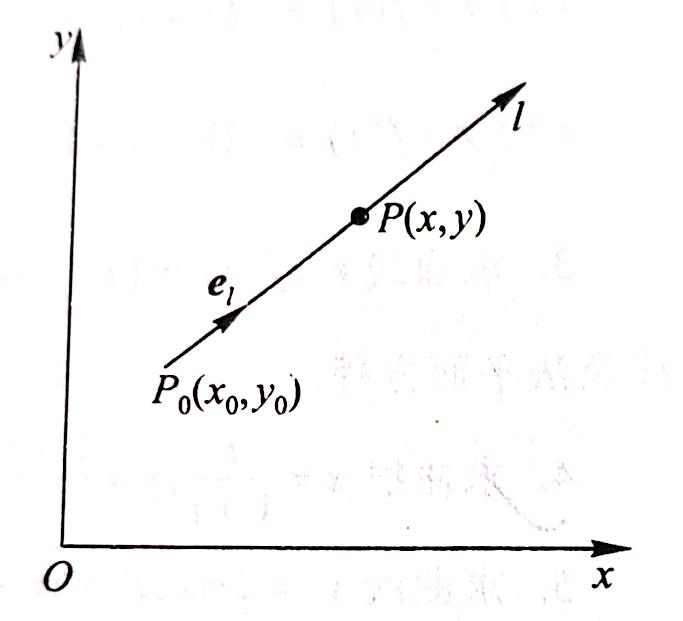
\includegraphics[scale=0.16]{Chapter 09 images/pic6.jpg}
    \]

    设\(l\)是\(xOy\)平面上以\(P_0\left(x_0,y_0\right)\)为始点的一条射线,
    \(\overrightarrow{e_1}=\left(\cos \alpha, \cos \beta\right)\)是与\(l\)同方向的单位向量。
    射线\(l\)的参数方程为

    \begin{equation}
        \left\{\begin{array}{l}
        x=x_0+t \cos \alpha \\
        y=y_0+t \cos \beta
        \end{array}(t \geq 0)\right.
    \end{equation}

    设函数\(z=f\left(x,y\right)\)在点\(P_0\left(x_0,y_0\right)\)的某个邻域
    \(U\left(P_0\right)\),\(P\left(x+t \cos \alpha,y+t \cos \beta\right)\)
    为\(l\)上另一点,且\(P \in U\left(P_0\right)\)。如果函数增量\(f\left(x+t \cos \alpha,y+t \cos \beta\right)-
    f\left(x_0,y_0\right)\)与\(P\)到\(P_0\)的距离\(\left|PP_0\right|=t\)的比值

    \begin{equation*}
        \frac{f\left(x_0+t \cos \alpha, y_0+t \cos \beta\right)-f\left(x_0, y_0\right)}{t}
    \end{equation*}

    当\(P\)沿着\(l\)趋于\(P_0\)(即\(t \rightarrow 0^{+}\))时的极限存在,那么称此极限为函数\(f\left(x,y\right)\)
    在\\\(P_0\left(x_0,y_0\right)\)处沿\(l\)的方向导数,
    记作\(\left.\dfrac{\partial f}{\partial l}\right|_{\left(x_0,y_0\right)}\),即

    \begin{equation}
        \left.\frac{\partial f}{\partial l}\right|_{\left(x_0, y_0\right)}=
        \lim_{t \rightarrow 0^{+}} \frac{f\left(x_0+t \cos \alpha, y_0+t \cos \beta\right)-f\left(x_0, y_0\right)}{t}
    \end{equation}

    方向导数\(\left.\dfrac{\partial f}{\partial l}\right|_{\left(x_0,y_0\right)}\)就是函数
    \(f\left(x,y\right)\)在点\(P_0\left(x_0,y_0\right)\)处沿方向\(l\)的变化率。
    
    若函数\(f\left(x,y\right)\)在点\(P_0\left(x_0,y_0\right)\)处的偏导数存在,
    取\(\overrightarrow{e}_l = \overrightarrow{i} = (1,0)\),则

    \begin{equation*}
        \left.\frac{\partial f}{\partial l}\right|_{\left(x_0, y_0\right)}=
        \lim _{t \rightarrow 0^{+}} \frac{f\left(x_0+t, y_0\right)-f\left(x_0, y_0\right)}{t}=f_x\left(x_0, y_0\right)
    \end{equation*}

    于是,我们有

    $$
        \text{偏导数存在} \Rightarrow \text{沿\(x\)轴正向的方向导数存在}
    $$

    同理,若取\(\overrightarrow{e}_l = \overrightarrow{j} = (0,1)\),则

    \begin{equation*}
        \left.\frac{\partial f}{\partial l}\right|_{\left(x_0, y_0\right)}=
        \lim _{t \rightarrow 0^{+}} \frac{f\left(x_0, y_0+t\right)-f\left(x_0, y_0\right)}{t}=f_y\left(x_0, y_0\right)
    \end{equation*}

    但反之,若\(\overrightarrow{e}_l = \overrightarrow{i}\),\(\left.\dfrac{\partial z}{\partial l}\right|_{\left(x_0,y_0\right)}\)
    存在,则\(\left.\dfrac{\partial z}{\partial x}\right|_{\left(x_0,y_0\right)}\)未必存在。

\subsubsection{计算公式}

    \textbf{定理}:如果函数\(f\left(x,y\right)\)在点\(P_0\left(x_0,y_0\right)\)可微分,
    那么函数在该点沿任意方向\(l\)的方向导数存在,且有

    \begin{equation}
        \left.\frac{\partial f}{\partial l}\right|_{\left(x_0, y_0\right)}=f_x\left(x_0, y_0\right) \cos \alpha+f_y\left(x_0, y_0\right) \cos \beta
    \end{equation}

    其中\(\cos \alpha\)和\(\cos \beta\)是方向\(l\)的方向余弦。

\subsubsection{推广}

    % \textbf{推广}

    对于三元函数\(f\left(x,y,z\right)\)来说,它在空间一点\(P_0\left(x_0,y_0,z_0\right)\)
    沿方向\\\(\overrightarrow{e}_l = \left(\cos \alpha, \cos \beta, \cos \gamma\right)\)的方向导数为

    \begin{equation}
        \left.\frac{\partial f}{\partial l}\right|_{\left(x_0, y_0, z_0\right)}=
        \lim _{t \rightarrow 0^{+}} \frac{f\left(x_0+t \cos \alpha, y_0+t \cos \beta, z_0
        +t \cos \gamma\right)-f\left(x_0, y_0, z_0\right)}{t}
        \end{equation}

    \textbf{定理}:如果函数\(f\left(x,y,z\right)\)在点\(P_0\left(x_0,y_0,z_0\right)\)可微分,
    那么函数在该点沿方向\\\(\overrightarrow{e}_l = \left(\cos \alpha, \cos \beta, \cos \gamma\right)\)的方向导数为

    \begin{equation}
        \left.\frac{\partial f}{\partial l}\right|_{\left(x_0, y_0, z_0\right)}=
        f_x\left(x_0, y_0, z_0\right) \cos \alpha+f_y\left(x_0, y_0, z_0\right) \cos \beta+
        f_z\left(x_0, y_0, z_0\right) \cos \gamma
    \end{equation}

\subsection{梯度}

\subsubsection{定义}

    设函数\(f\left(x,y\right)\)在平面区域\(D\)内具有一阶连续偏导数,则对每一点
    \(P_0\left(x_0,y_0\right) \in D\),都可定出一个向量

    \begin{equation}
        f_x\left(x_0, y_0\right) \overrightarrow{i}+f_y\left(x_0, y_0\right) \overrightarrow{j}
    \end{equation}

    这向量称为函数\(f\left(x,y\right)\)在点\(P_0\left(x_0,y_0\right) \in D\)的梯度,
    记作\(\operatorname{grad} f\left(x_0,y_0\right)\)或\(\nabla f\left(x_0,y_0\right)\),
    即

    \begin{equation}
        \operatorname{grad} f\left(x_0, y_0\right)=\nabla f\left(x_0, y_0\right)=
        f_x\left(x_0, y_0\right) \overrightarrow{i}+f_y\left(x_0, y_0\right) \overrightarrow{j}
    \end{equation}

    其中$\nabla=\dfrac{\partial}{\partial x} \overrightarrow{i}+\dfrac{\partial}{\partial y} \overrightarrow{j}$
    称为(二维的)向量微分算子或Nabla算子,
    $\nabla f=\dfrac{\partial f}{\partial x} \overrightarrow{i}+\dfrac{\partial f}{\partial y} \overrightarrow{j}$

    \textbf{推广}:

    $$
        \nabla f\left(x_0, y_0, z_0\right)=\left(f_x\left(x_0, y_0, x_0\right),
        f_y\left(x_0, y_0, z_0\right), f_z\left(x_0, y_0, z_0\right)\right) .
    $$

\subsubsection{梯度与方向导数的关系}

    如果函数\(f\left(x,y\right)\)在点\(P_0\left(x_0,y_0\right)\)处可微分,
    \(\overrightarrow{e}_l=\left(\cos \alpha, \cos \beta\right)\)是与\(l\)同方向的单位向量,那么

    \begin{equation}
        \begin{aligned}
        \left.\frac{\partial f}{\partial l}\right|_{\left(x_0, y_0\right)} & =f_x\left(x_0, y_0\right) \cos \alpha+f_y\left(x_0, y_0\right) \cos \beta \\
        & =\operatorname{grad} f\left(x_0, y_0\right) \cdot \overrightarrow{e}_l=\left|\operatorname{grad} f\left(x_0, y_0\right)\right| \cos \theta
        \end{aligned}
    \end{equation}

    其中$\theta=\left(\operatorname{grad} \widehat{f\left(x_0, y_0\right), \overrightarrow{e}_l}\right)$

    \begin{enumerate}
        \item 当\(\theta=0\),即方向\(\overrightarrow{e}_l\)与\(\operatorname{grad} f\left(x_0, y_0\right)\)一致时,
            函数\(f\left(x,y\right)\)增长最快。此时,函数在这个方向导数达到最大值,这个最大值就是梯度
            \(\operatorname{grad} f\left(x_0, y_0\right)\)的模,即
            $$
                \left.\frac{\partial f}{\partial l}\right|_{\left(x_0, y_0\right)}=
                \left|\operatorname{grad} f\left(x_0, y_0\right)\right|
            $$
            函数\(f\left(x,y\right)\)在点\(P_0\left(x_0,y_0\right)\)的梯度\(\operatorname{grad} f\)的方向是函数在这点的方向导数取得最大值的方向,
            它的模就等于最大值。
        \item 当\(\theta=\uppi\),即方向\(\overrightarrow{e}_l\)与\(\operatorname{grad} f\left(x_0, y_0\right)\)相反时,
            函数\(f\left(x,y\right)\)减少最快,函数在这个方向导数达到最小值,即
            $$
                \left.\frac{\partial f}{\partial l}\right|_{\left(x_0, y_0\right)}=-\left|\operatorname{grad} f\left(x_0, y_0\right)\right|
            $$
        \item 当\(\theta=\frac{\uppi}{2}\),即方向\(\overrightarrow{e}_l\)与\(\operatorname{grad} f\left(x_0, y_0\right)\)正交时,
            函数的变换率为0,即
            $$
                \left.\frac{\partial f}{\partial l}\right|_{\left(x_0, y_0\right)}=\left|\operatorname{grad} f\left(x_0, y_0\right)\right| \cos \theta=0 .
            $$
    \end{enumerate}

\subsubsection{梯度与等值线的关系}

    二元函数\(z=f\left(x,y\right)\)在几何上表示一个曲面,这曲面被平面\(z=c\)(\(c\)是常数)所截得的曲线\(L\)的方程为

    $$
        \left\{\begin{array}{l}
            z=f(x, y) \\
            z=c
        \end{array}\right.
    $$

    \[
        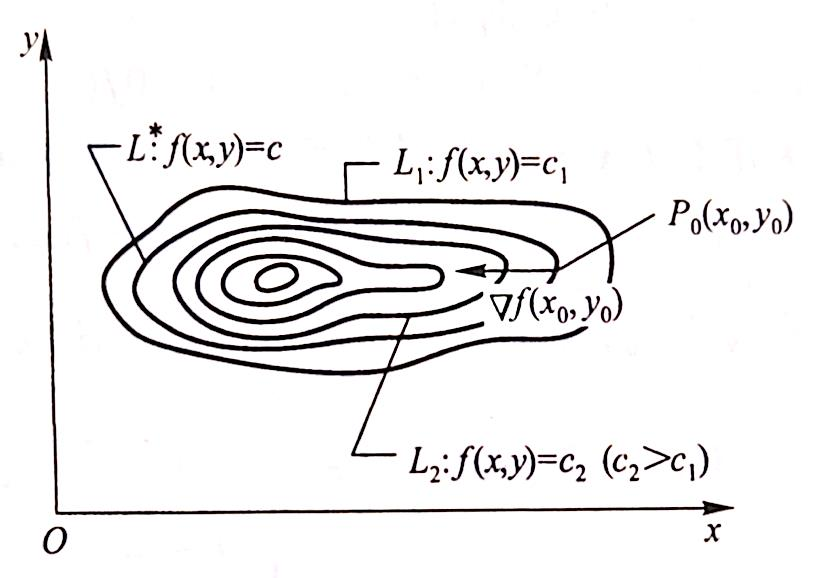
\includegraphics[scale=0.2]{Chapter 09 images/pic7.jpg}
    \]

    这条曲线\(L\)在\(xOy\)面上的投影是一条平面曲线\(L^{*}\),它在\(xOy\)
    平面直角坐标系中的方程为

    \[
        f\left(x,y\right) = c
    \]

    对于曲线\(L^{*}\)上的一切点,已给函数的函数值都是\(c\),
    所以我们称平面曲线\(L^{*}\)为函数\(z=f\left(x,y\right)\)的等值线。

    若\(f_x\)、\(f_y\)不同时为零,则等值线\(f\left(x,y\right) = c\)
    上任一点\(P_0\left(x_0,y_0\right)\)处的一个单位法向量为

    \begin{equation}
        \begin{aligned}
            \overrightarrow{n} & =\frac{1}{\sqrt{f_x^2\left(x_0, y_0\right)+f_y^2\left(x_0, y_0\right)}}\left(f_x\left(x_0, y_0\right), f_y\left(x_0, y_0\right)\right) \\
            & =\frac{\nabla f\left(x_0, y_0\right)}{\left|\nabla f\left(x_0, y_0\right)\right|}
        \end{aligned}
    \end{equation}

    说明函数\(z=f\left(x,y\right)\)在\(\left(x_0,y_0\right)\)处的梯度方向就是\(f\left(x,y\right) = c\)
    在该点处的法线方向\(\overrightarrow{n}\),且

    \begin{equation}
        \nabla f\left(x_0, y_0\right)=\frac{\partial f}{\partial n} \overrightarrow{n}
    \end{equation}

\subsubsection{数量场、向量场}

    \begin{enumerate}
        \item \(M \in G\),数量\(f\left(M\right)\):数量场(如温度场、密度场)
        \item \(M \in G\),向量\(\overrightarrow{F}\left(M\right)\):向量场(如力场、速度场)
            $$
                \overrightarrow{F}(M)=P(M) \overrightarrow{i}+Q(M) \overrightarrow{j}+R(M) \overrightarrow{k}
            $$
        \item 若向量场\(\overrightarrow{F}\left(M\right)\)是某个数量函数\(f\left(M\right)\)的梯度,
            则称\(f\left(M\right)\)是\(\overrightarrow{F}\left(M\right)\)的一个势函数,\\并称
            \(\overrightarrow{F}\left(M\right)\)为势场。
    \end{enumerate}

\section{多元函数的极值及其求法}

\subsection{多元函数的极值及其最大值与最小值}

\subsubsection{极值的定义}

    设函数\(z=f\left(x.y\right)\)的定义域为\(D\),\(P_0\left(x_0,y_0\right)\)为\(D \)的内点。
    若存在\(P_0\)的某个邻域\(U\left(P_0\right) \subset D\),使得对于该邻域内异于\(P_0\)的任何点\(\left(x,y\right)\),
    都有

    \[
        f\left(x,y\right) < f\left(x_0,y_0\right)
    \]

    则称函数\(f\left(x.y\right)\)在点\(\left(x_0,y_0\right)\)有极大值\(f\left(x_0,y_0\right)\),
    点\(\left(x_0,y_0\right)\)称为函数\(f\left(x.y\right)\)的极大值点;
    
    
    若对于该邻域内异于\(P\)的任何点\(\left(x,y\right)\),都有
    
    \[
        f\left(x,y\right) < f\left(x_0,y_0\right)
    \]

    则称函数\(f\left(x.y\right)\)在点\(\left(x_0,y_0\right)\)有极小值\(f\left(x_0,y_0\right)\),
    点\(\left(x_0,y_0\right)\)称为函数\(f\left(x.y\right)\)的极小值点;

    极大值与极小值统称为极值,使得函数取得极值的点称为极值点。

    \textbf{注意}:

    \begin{enumerate}
        \item \(f \)在极值点的邻域内有定义,但不一定在该点连续;
        \item 极值是局部最值;
        \item 类似可定义多元函数极值。
    \end{enumerate}
 
\subsubsection{极值的条件}
    
    \textbf{定理1}(必要条件):设函数\(z=f\left(x.y\right)\)在点\(\left(x_0,y_0\right)\)具有偏导数,
    且在点\(\left(x_0,y_0\right)\)处有极值,则有

    \begin{align}
        f_x\left(x_0,y_0\right) = 0, f_y\left(x_0,y_0\right) = 0
    \end{align}

    \textbf{注意}:

    \begin{enumerate}
        \item 称使得\(f_x\left(x_0,y_0\right) = 0, f_y\left(x_0,y_0\right) = 0\)的点称为\(f\left(x.y\right)\)的驻点;
        \item 几何解释:曲面\(z=f\left(x.y\right)\)在极值点对应点\(\left(x_0,y_0,f\left(x_0,y_0\right)\right)\)
            处的切平面法向量
            $$
                \overrightarrow{n}=\left(f_x\left(x_0, y_0\right), f_y\left(x_0, y_0\right),-1\right)=(0,0,-1)
            $$
            平行于\(z\)轴,故切平面平行于\(xOy\)面(水平);
        \item 类似可推广到多元函数的极值。
    \end{enumerate}

    \textbf{定理2}(充分条件):设函数\(z=f\left(x.y\right)\)在点\(\left(x_0,y_0\right)\)
    的某个邻域内连续且有一阶及二阶连续偏导数,有\(f_x\left(x_0,y_0\right) = 0\),
    \(f_y\left(x_0,y_0\right) = 0\),令

    $$
        f_{x x}\left(x_0, y_0\right)=A, f_{x y}\left(x_0, y_0\right)=B, f_{y y}\left(x_0, y_0\right)=C
    $$

    则\(f\left(x,y\right)\)在点\(\left(x_0,y_0\right)\)处是否取得极值的条件如下;

    \begin{enumerate}
        \item \(AC - B^2>0\)时具有极值,且当\(A<0\)时有极大值,且当\(A>0\)时有极小值;
        \item \(AC - B^2>0\)时没有极值;
        \item \(AC - B^2=0\)时可能有极值,也可能没有极值,还需另作讨论;
    \end{enumerate}

\subsubsection{最值问题}

    求函数\(z=f\left(x.y\right)\)在闭区域\(D \)上的最值。(\(f \)在\(D \)上连续,在\(D \)内可微且只有有限个驻点)

    \begin{enumerate}
        \item 求\(f \)在\(D \)内的全部驻点;
        \item 求\(f \)在\(D \)上的最值点;
        \item 将1、2中的点函数值进行比较。
    \end{enumerate}

    实际问题中,若已知最值必在内部取得,且驻点位移,
    则驻点就是所求最值点。

\end{document}
